\documentclass[preprint]{aastex}   % one column
%\documentclass[preprint2]{aastex}  % two columns
\usepackage[margin=1.5in]{geometry}
\setlength{\parindent}{0em}
\setlength{\parskip}{0.75ex}
\usepackage{graphicx}
\usepackage{enumitem}
\usepackage{amsmath}
\usepackage{xcolor}

\usepackage{natbib}
%\usepackage{booktabs}  % ??
\bibliographystyle{apj}

\usepackage{titlesec}
%\titlespacing*{⟨command⟩}{⟨left⟩}{⟨before-sep⟩}{⟨after-sep⟩}[⟨right-sep⟩]
%\titlespacing*{\section}{-0.5in}{0ex}{0ex}
%\titlespacing*{\subsection}{0pt}{0.5ex}{-10ex}

\usepackage{url}
\usepackage{hyperref}
\definecolor{darkblue}{rgb}{0.0, 0.2, 0.6}
\definecolor{darkred}{rgb}{0.8, 0.0, 0.0}
\hypersetup{colorlinks=true,
    citecolor=darkblue,
    urlcolor=darkblue,
    linkcolor=black }
\urlstyle{same}

\shorttitle{Bright Point Size}
\shortauthors{Farris}

%
%
%
%

\begin{document}

\title{Determining coronal bright point size via cross-correlation using
multi-wavelength images from AIA/\textit{SDO}}
\author{Laurel Farris, R. T. James McAteer}
\affil{New Mexico State University}
\email{laurel07@nmsu.edu}

\begin{abstract}
Coronal bright points are observed in a relatively uniform distribution across the
solar disk in the X-ray and EUV wavelength regimes.
Here,
\end{abstract}
\keywords{Sun: corona{-}Sun: bright points{-}Sun: multi-wavelength}

\section{Introduction}\label{intro}


\subsection{General information}
% How observed
Coronal bright points (CBPs)
are observed ubiquitously in the solar atmosphere in the X-ray and EUV
wavelength regimes, with a spatial distribution that becomes more homogeneous
and numerous during solar minimum (\cite{Priest}).
Though they only cover about 1.6\% of the
photosphere (\cite{Srivastava}), CBPs and sunspots
contribute over 90\% of the total magnetic flux (\cite{Howard}).
Over the course of the solar cycle, they can contribute significantly to the
global intensity variation of the sun, particularly in the ultraviolet
regime (\cite{Riethmuller}).

% What they are
CBPs are thought to be composed of bundles of coronal loops, and
consist of two components: a bright center and a surrounding darker
region (\cite{Zhang}; \cite{Alipour}).
Flashes of emission, or ``jets'' have been observed around these CBPs, with
characteristic periods of about one hour (\cite{Zhang}).

\subsection{Previous size determination methods}
Several techniques for determining the size of coronal CBPs have been employed
in the literature.
\cite{Alipour}
developed an algorithm to locate CBPs in the corona, using size determined
by intensity as part of the criteria for distinguishing CBPs from other features,
such as top-down views of coronal loops or nanoflares.


\subsection{Outline of current project}
Here, the size of a single CBP was determined using cross-correlation techniques.
The data is described in \S{}\ref{data},
the results are examined in \S{}\ref{results},
with a subsequent analysis in \S{}\ref{analysis},
and the primary conclusions are discussed in \S{}\ref{conclusion}.


\section{Data}\label{data}

\subsection{Download}
This study used
multi-wavelength data from AIA/\textit{SDO}
spanning one hour on June 1, 2012 from 13:00:00 to 13:59:59, at a cadence of 12
seconds.
The relevant values for each passband are given in table \ref{temps}.

\begin{table}[h]
\centering
    \begin{tabular}{l l l}
        \hline\hline
        $\lambda$ [\AA{}] & log(T) [K] & Ion \\
        \hline
        94 & 6.8 & Fe {\small XVIII} \\
        131 & 5.6, 7.0 & Fe {\small VIII, XXI} \\
        171 & 5.8 & Fe {\small IX} \\
        193 & 6.2, 7.3 & Fe {\small XII, XXIV} \\
        211 & 6.3 & Fe {\small XIV} \\
        304 & 4.7 & He {\small II} \\
        335 & 6.4 & Fe {\small XVI} \\
    \end{tabular}
\caption{Characteristic temperatures corresponding to the wavelengths observed
    in emission in the solar corona (from \cite{Lemen}).}
\label{temps}
\end{table}

The data was downloaded using \verb|vsoget.pro|, a procedure that
both queries and/or downloads data from any of the three instruments on SDO.
The downloaded data was processed at level 1.0.
\textcolor{darkred}{Double check difference between 1.0 and 1.5 and see if this
is important\ldots}

A grayscale image of the full disk at the beginning of the time series for each
pass band is shown in figure \ref{full}.
A single CBP was selected from the coronal hole in the upper
left region of the solar disk.
100 pixel$^{2}$ ($\sim$ 60 arcsecond$^{2}$)
images of this BP in each passband are shown in figure \ref{bp_images}.
As noted by \cite{Alipour} in their study, the CBP structure is most evident for the
131\AA{}, 193\AA{}, and 211\AA{} images.


\subsection{Reading and/or restoring of data and header information}
The \verb|read_sdo.pro| routine from solar software (ssw)
\textcolor{darkred}{(source?)} was used to read the data and headers from the
fits files.
Since the header information was read into structures, it was necessary to
read them at the start of every run since
variables in structure form evidently cannot
easily (if at all) be saved and restored as \verb|.sav| files.
For simplicity, an alternative was not explored since reading headers
alone did not take a significant amount of time.

I wrote a code called \verb|bp_read_my_fits.pro| with the option to read
data from the fits files or from saved variables (\verb|*.sav|) if the data had
already been read and processed (see \S\ref{ssec:align}), as well as read
the headers into a separate variable.
The pass bands of interest were entered as an input variable in the form of
a string array, e.g. [`171', `193'].
To provide the most efficient means of reading and organizing the wealth of
required information, this code created
a separate structure for each pass band
into which the desired data range, central wavelength,
cross-correlation values, and other pertinent information from the headers was written.
In addition to making the task of re-reading data and adding extra header information
as quick and simple as possible, this code was written as a general means of
reading and organizing any future data, regardless of instrument or location.


\subsection{Processing: alignment}\label{ssec:align}
Before analysis, an alignment procedure called \verb|align_cube3.pro|
was run on each data cube. This
involved choosing a reference image (in this case, the image halfway through
the time series) for every other image to be aligned to. This procedure
corrected for shifts between images due to instrumental effects or the global
rotation of the sun.

Each shift resulted in the pixels at the edges of the data array to wrap around
to the opposite side in both the x and y dimensions. Therefore, it was necessary
to run the alignment on a larger two-dimensional data set than just the portion
needed for analysis.

The amount by which an image shifted each time was determined by the routine
\verb|alignoffset.pro| and returned as a 2xN array (where N = number of images)
called ``offsets'' (in x and y).
This procedure was quite mathy and I made no attempt to figure out how it worked.
These offsets generally started at 2-3 pixels, then after several
runs through the procedure, went down to the sub-pixel level.

The routine \verb|shift_sub.pro|, another mathy code, was then called by
\verb|align_cube3.pro| to do the actual shifting of each image, down to
sub-pixel accuracies. An interpolated image was returned if the difference
was greater than one pixel. If the difference was less than one pixel,
the actual values of the offsets determined the amount by which the cube
was shifted.

The repetitions
were halted as soon as the amount of shift ceased to change by a significant
amount (which was determined using the standard deviation so as to account for
negative values as the image shifted back and forth). At this point, the data
cube was deemed ``sufficiently aligned'' and ready for analysis.

All three procedures mentioned above were acquired courtesy of Dr. McAteer
and Dr. Gallagher.



\begin{figure*}[htb!]
    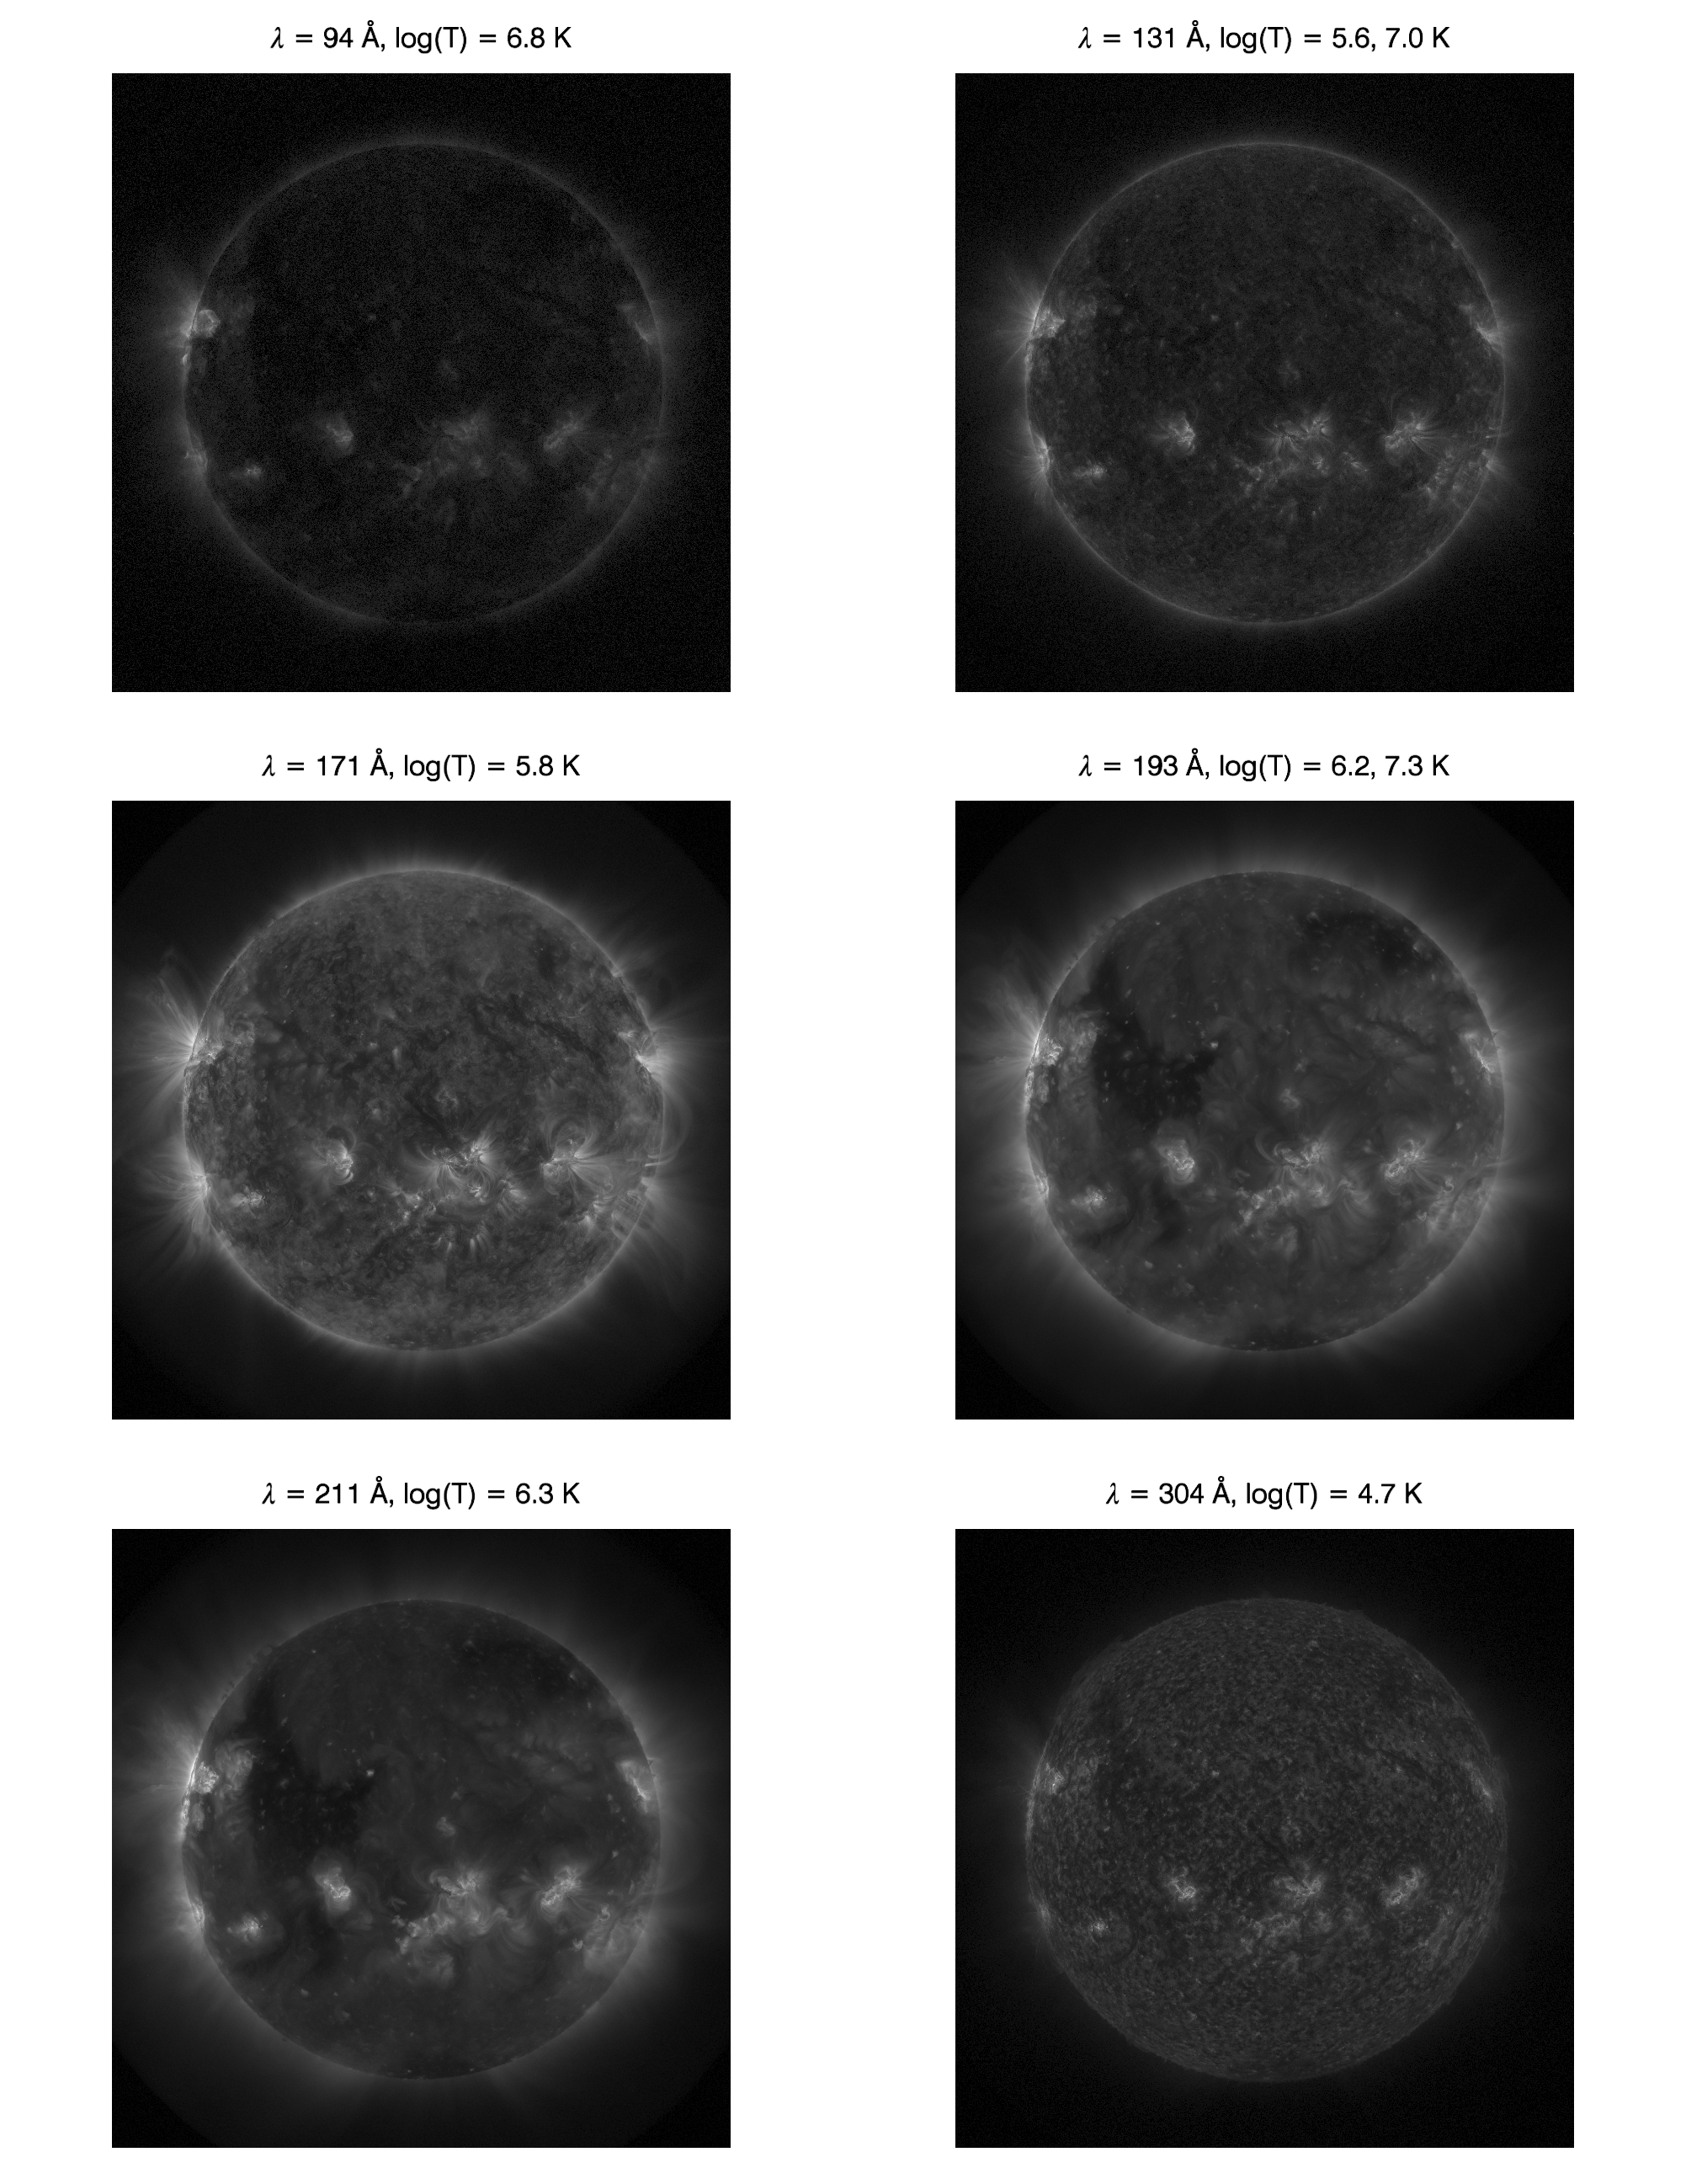
\includegraphics[width=\textwidth]{Figures/images/full_all.png}
    \caption{Full disk showing the relative intensity at the start of the time
        series for each AIA bandpass used in this study. These images show the
        square root of the exact data values for better visualization of the features. }
    \label{full}
\end{figure*}

\begin{figure*}[htb!]
    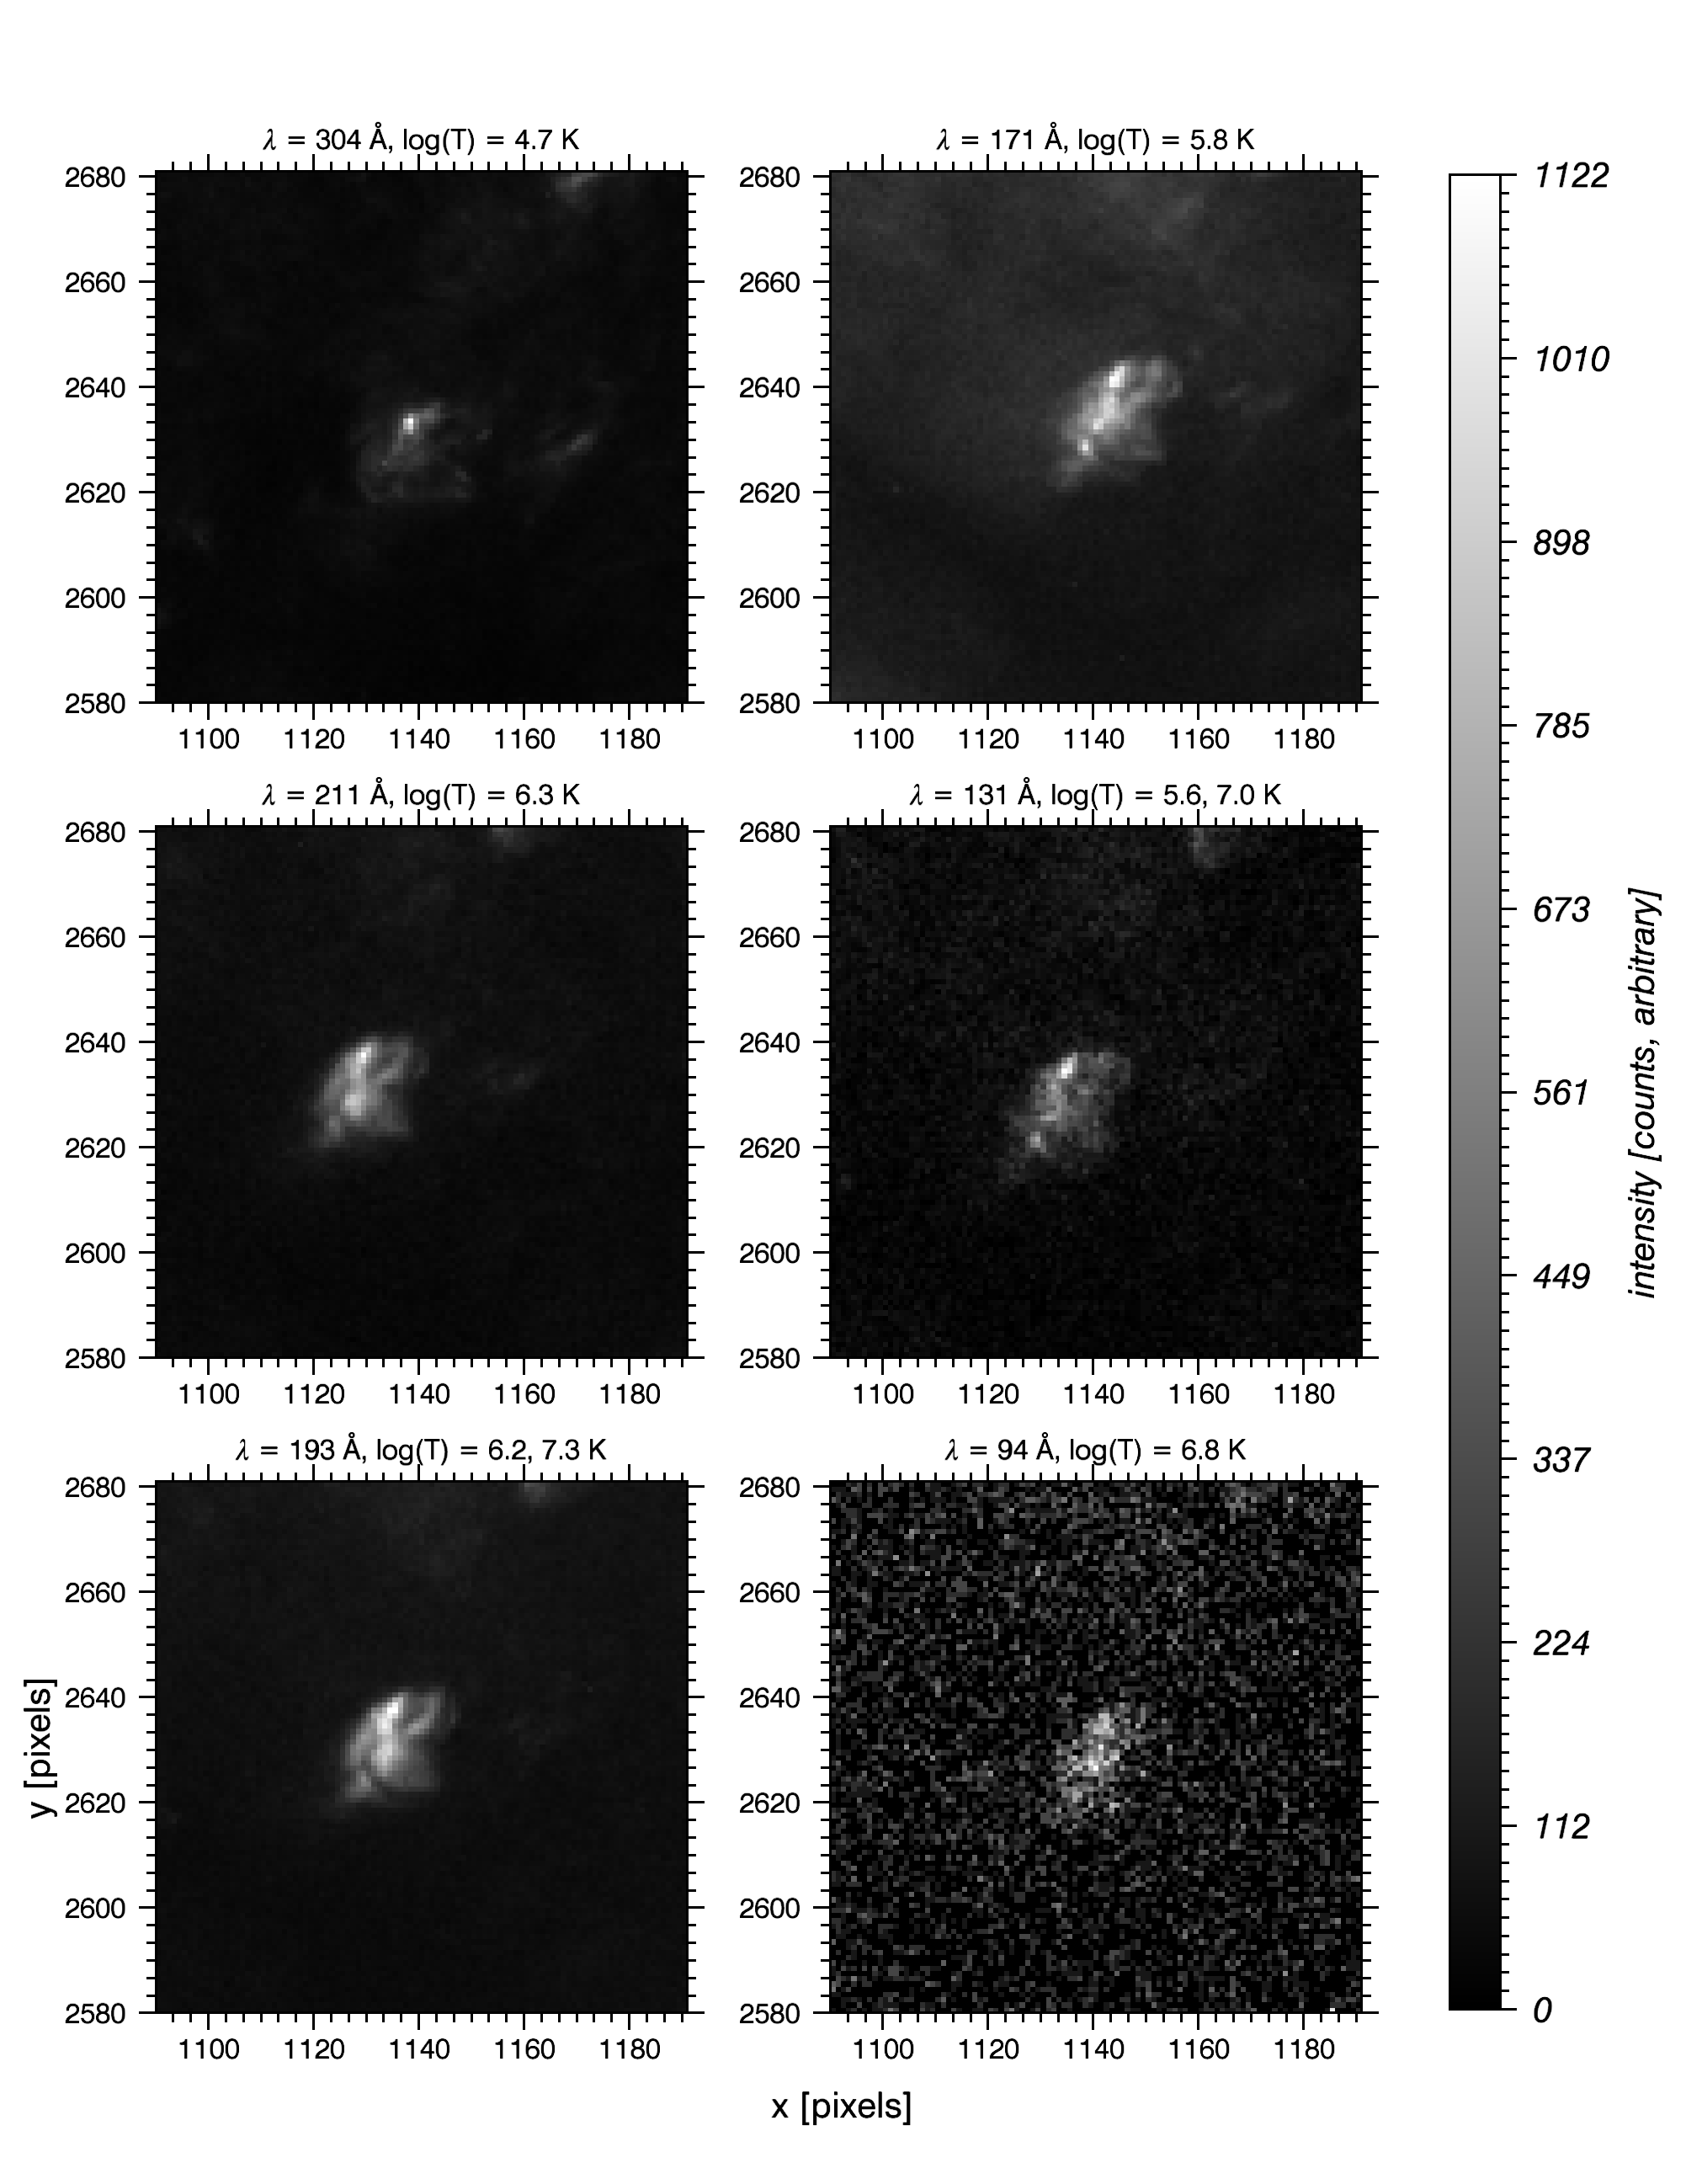
\includegraphics[width=\textwidth]{Figures/images/bp_all.png}
    \caption{Images of the BP in six different AIA wavelengths. The pixel coordinates
        are given relative to the full disk shown in figure \ref{full}. The
        location of the BP appears to shift from one bandpass to next, which
        may indicate a structure that is not completely straight, or a possible
        shift in the data itself. As with figure \ref{full}, these images show
        the square root of the original data values.}
    \label{bp_images}
\end{figure*}



\section{Analysis}\label{analysis}
\subsection{Cross-correlation}\label{cross-correlation}
\subsubsection{General definition}

The cross-correlation of two functions gives a quantitative value of how
``similar'' the two functions are. This similarity is given as a function of the
``lag'' between the two functions, i.e. the phase shift between the two functions
at which a given correlation value occurs. (\textcolor{darkred}{Source?})
Mathematically, the cross-correlation between two functions, $f$ and $g$, is
given by
\begin{equation}
    ( f \star g )(\tau) \equiv \int{ f(t)^{*} g(t-\tau) \mathrm{d}t }
\end{equation}
where $\tau$ is the lag between the two functions. If $\tau$ is positive, then

In statistical applications, the \textit{normalized} cross-correlation is calculated,
giving a rage of possible values
between -1 and +1, where a value of
+1 means the two functions are exactly correlated, a value of
-1 means the two functions are \emph{anti}-correlated,
and a value of 0 implies no correlation at all.

The complex conjugate of $f(t)$ in the integral ensures that the peaks/troughs
of a complex function will align in a way that contributes positive values to the
integral (otherwise the correlation values will be the opposite of what they
should be\ldots?).


\subsubsection{Application to BP size}

The procedure \verb|timelag.pro| normalized the cross-correlation values
to account for instrumental effects and the fact that the intensity values
from \textit{SDO}/AIA data are not physical.
\textcolor{darkred}{Between -1 and 1 or between 0 and 1 ??}
As a result, the absolute intensity values did not have an effect on how
well any two given light curves were correlated. Only the relative intensity,
i.e. the actual pattern of the light curves was considered.
This code took two light curves at a time, which here was two individual pixels, varying in
time but static in space.

The array of possible timelags was given as
$-\tau/2 \rightarrow \tau/2$, rather than
$0 \rightarrow \tau$.
This was because, while in principle the two curves are shifted past each other into
space where the other doesn't exist (and hence gives a value of zero),
the code causes the endpoints of the shifted function to wrap around to the
opposite end and be calculated by the initial function as it actually exists
in that space. Therefore, the function is shifted forward by half of the full
range in $\tau$, and then backward (from the original position) by half of the full
range again. This has the effect of maximum correlation values having corresponding
timelags that can be either negative or positive. A positive lag means the first
function actually ``leads'' the second by $\tau$, whereas a negative lag means the
first function ``lags'' the second (seems kind of backward, but whatev.)

The array of possible timelags was initially given simply as the image index in
the series (0 to 299), but the observation time from the header was substituted
later as a more physical shift between each time series.

It should be noted that the full length of the time series (one hour) was chosen to
ensure a good buffer around the amount of time over which a disturbance could travel
an appreciable distance across the approximate size scale of BPs (``size'' being
determined from previous literature and based roughly on intensity relative to the
background in a single image).

For an initial look at the type of results to be expected, a pixel roughly in the center
of the BP was chosen arbitrarily based on
the intensity of the initial image in each time series. The cross-correlation procedure was
run over the time series of this pixel and every other pixel in the 100 pixel$^{2}$ data
cube. There are several relationships that can be examined here.
The correlation values between two curves as a function of timelag is the standard
output from two single functions. One generally sees a bell-shaped curve whose
peak y-value occurs at some value $\tau_{max}$ on the x-axis. This peak is the maximum
correlation between the two curves, and $\tau_{max}$ is the lag that occurs between the
points where they are most highly correlated.

The purpose of the cross-correlation analysis was to help
determine, at the lowest possible resolution, which parts of the BP were moving
together as a single physical structure. The timelag at which the highest correlation
occurs was expected to be of the same order as the acoustic crossing time.
Since
magnetism dominates the behavior of waves produced in the solar corona, the
speed at which a wave moves through a feature there is expected
to be close to that of the characteristic Alfv\'en speed.

The intensity of each BP compared to the background flux surrounding it
can give a visual estimate
of its size. The intensity of the first image in each
passband is plotted as a function of radial distance from the central pixel in figures
\ref{intensity_1} and \ref{intensity_2}.


\section{Results and discussion}\label{results}
Images illustrating the highest cross-correlation value of each pixel and the
timelag corresponding to that correlation value are shown in figures \ref{cc_all}
and \ref{tt_all}, respectively. A color variation of the correlation images
is also shown (figure \ref{cc_all_color}).

\begin{figure*}[htb!]
    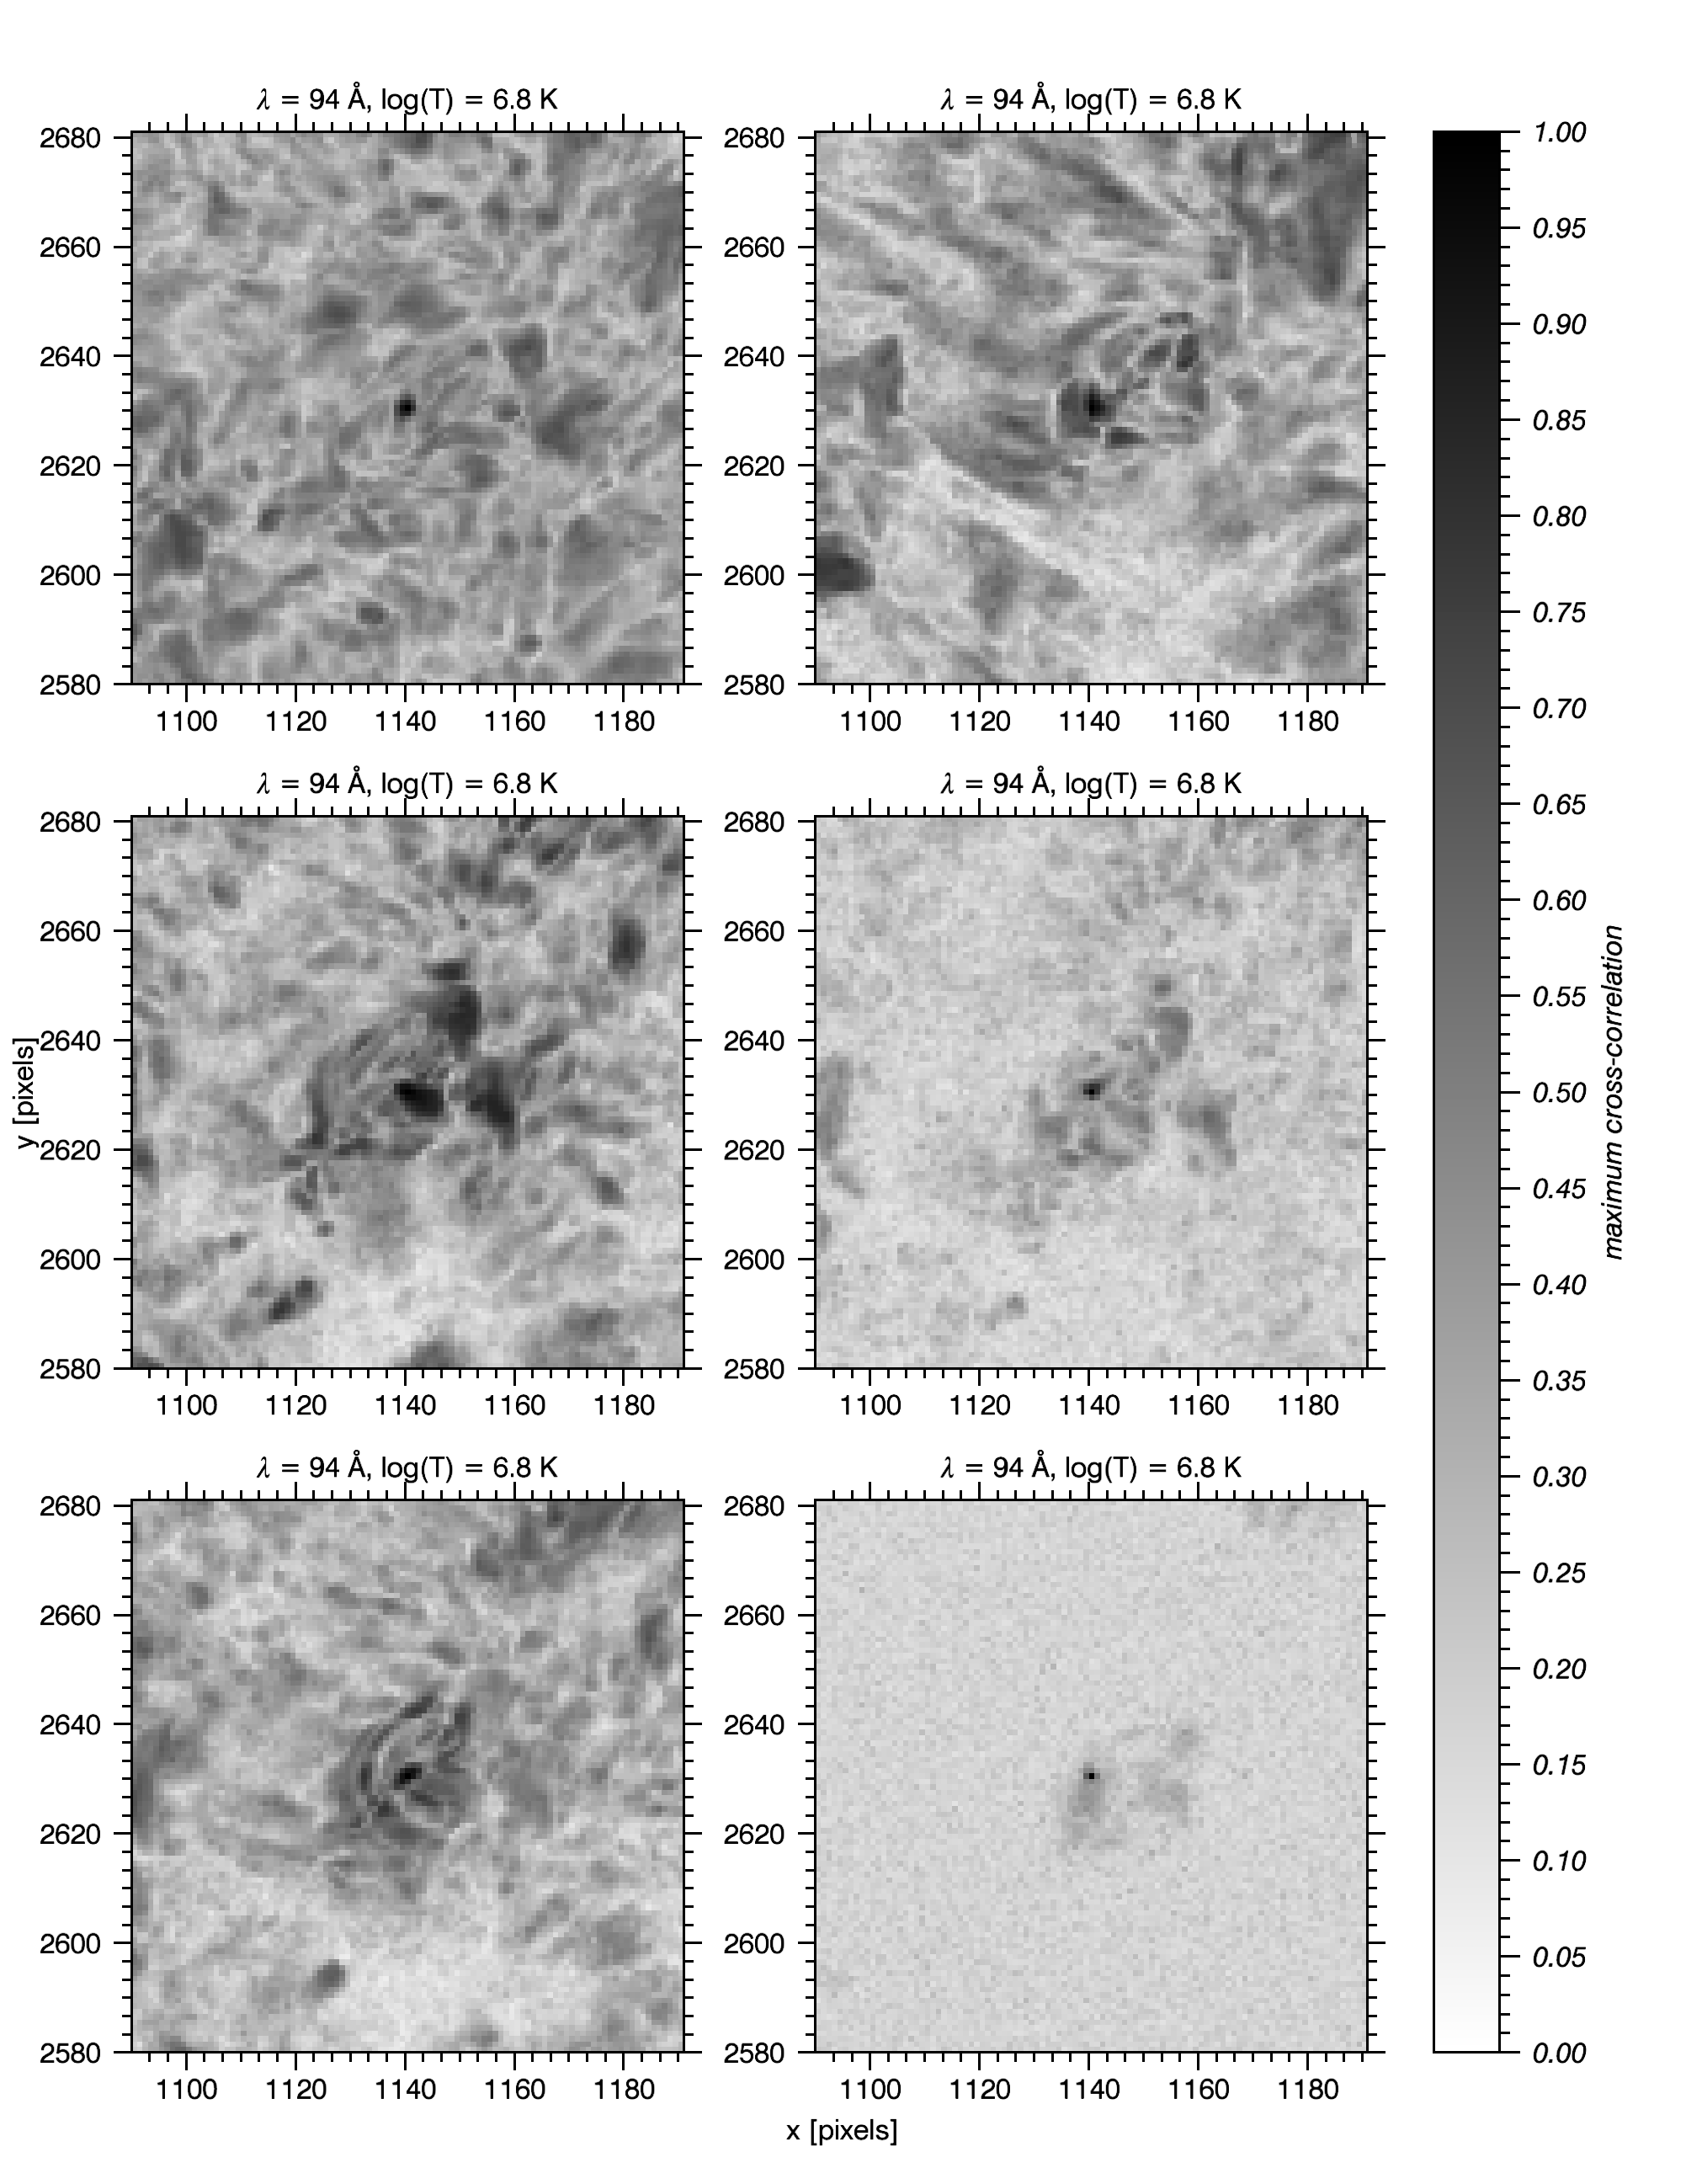
\includegraphics[width=\textwidth]{Figures/cc_images/cc_all_grayscale.png}
    \caption{Images showing the highest cross-correlation value for each pixel. }
    \label{cc_all}
\end{figure*}

The correlation was given a threshold of 0.5 and rescaled to obtain a
better illustration of the structure of the BP. These images are shown in
figures \ref{cc} and \ref{tt}.

\begin{figure*}[htb!]
    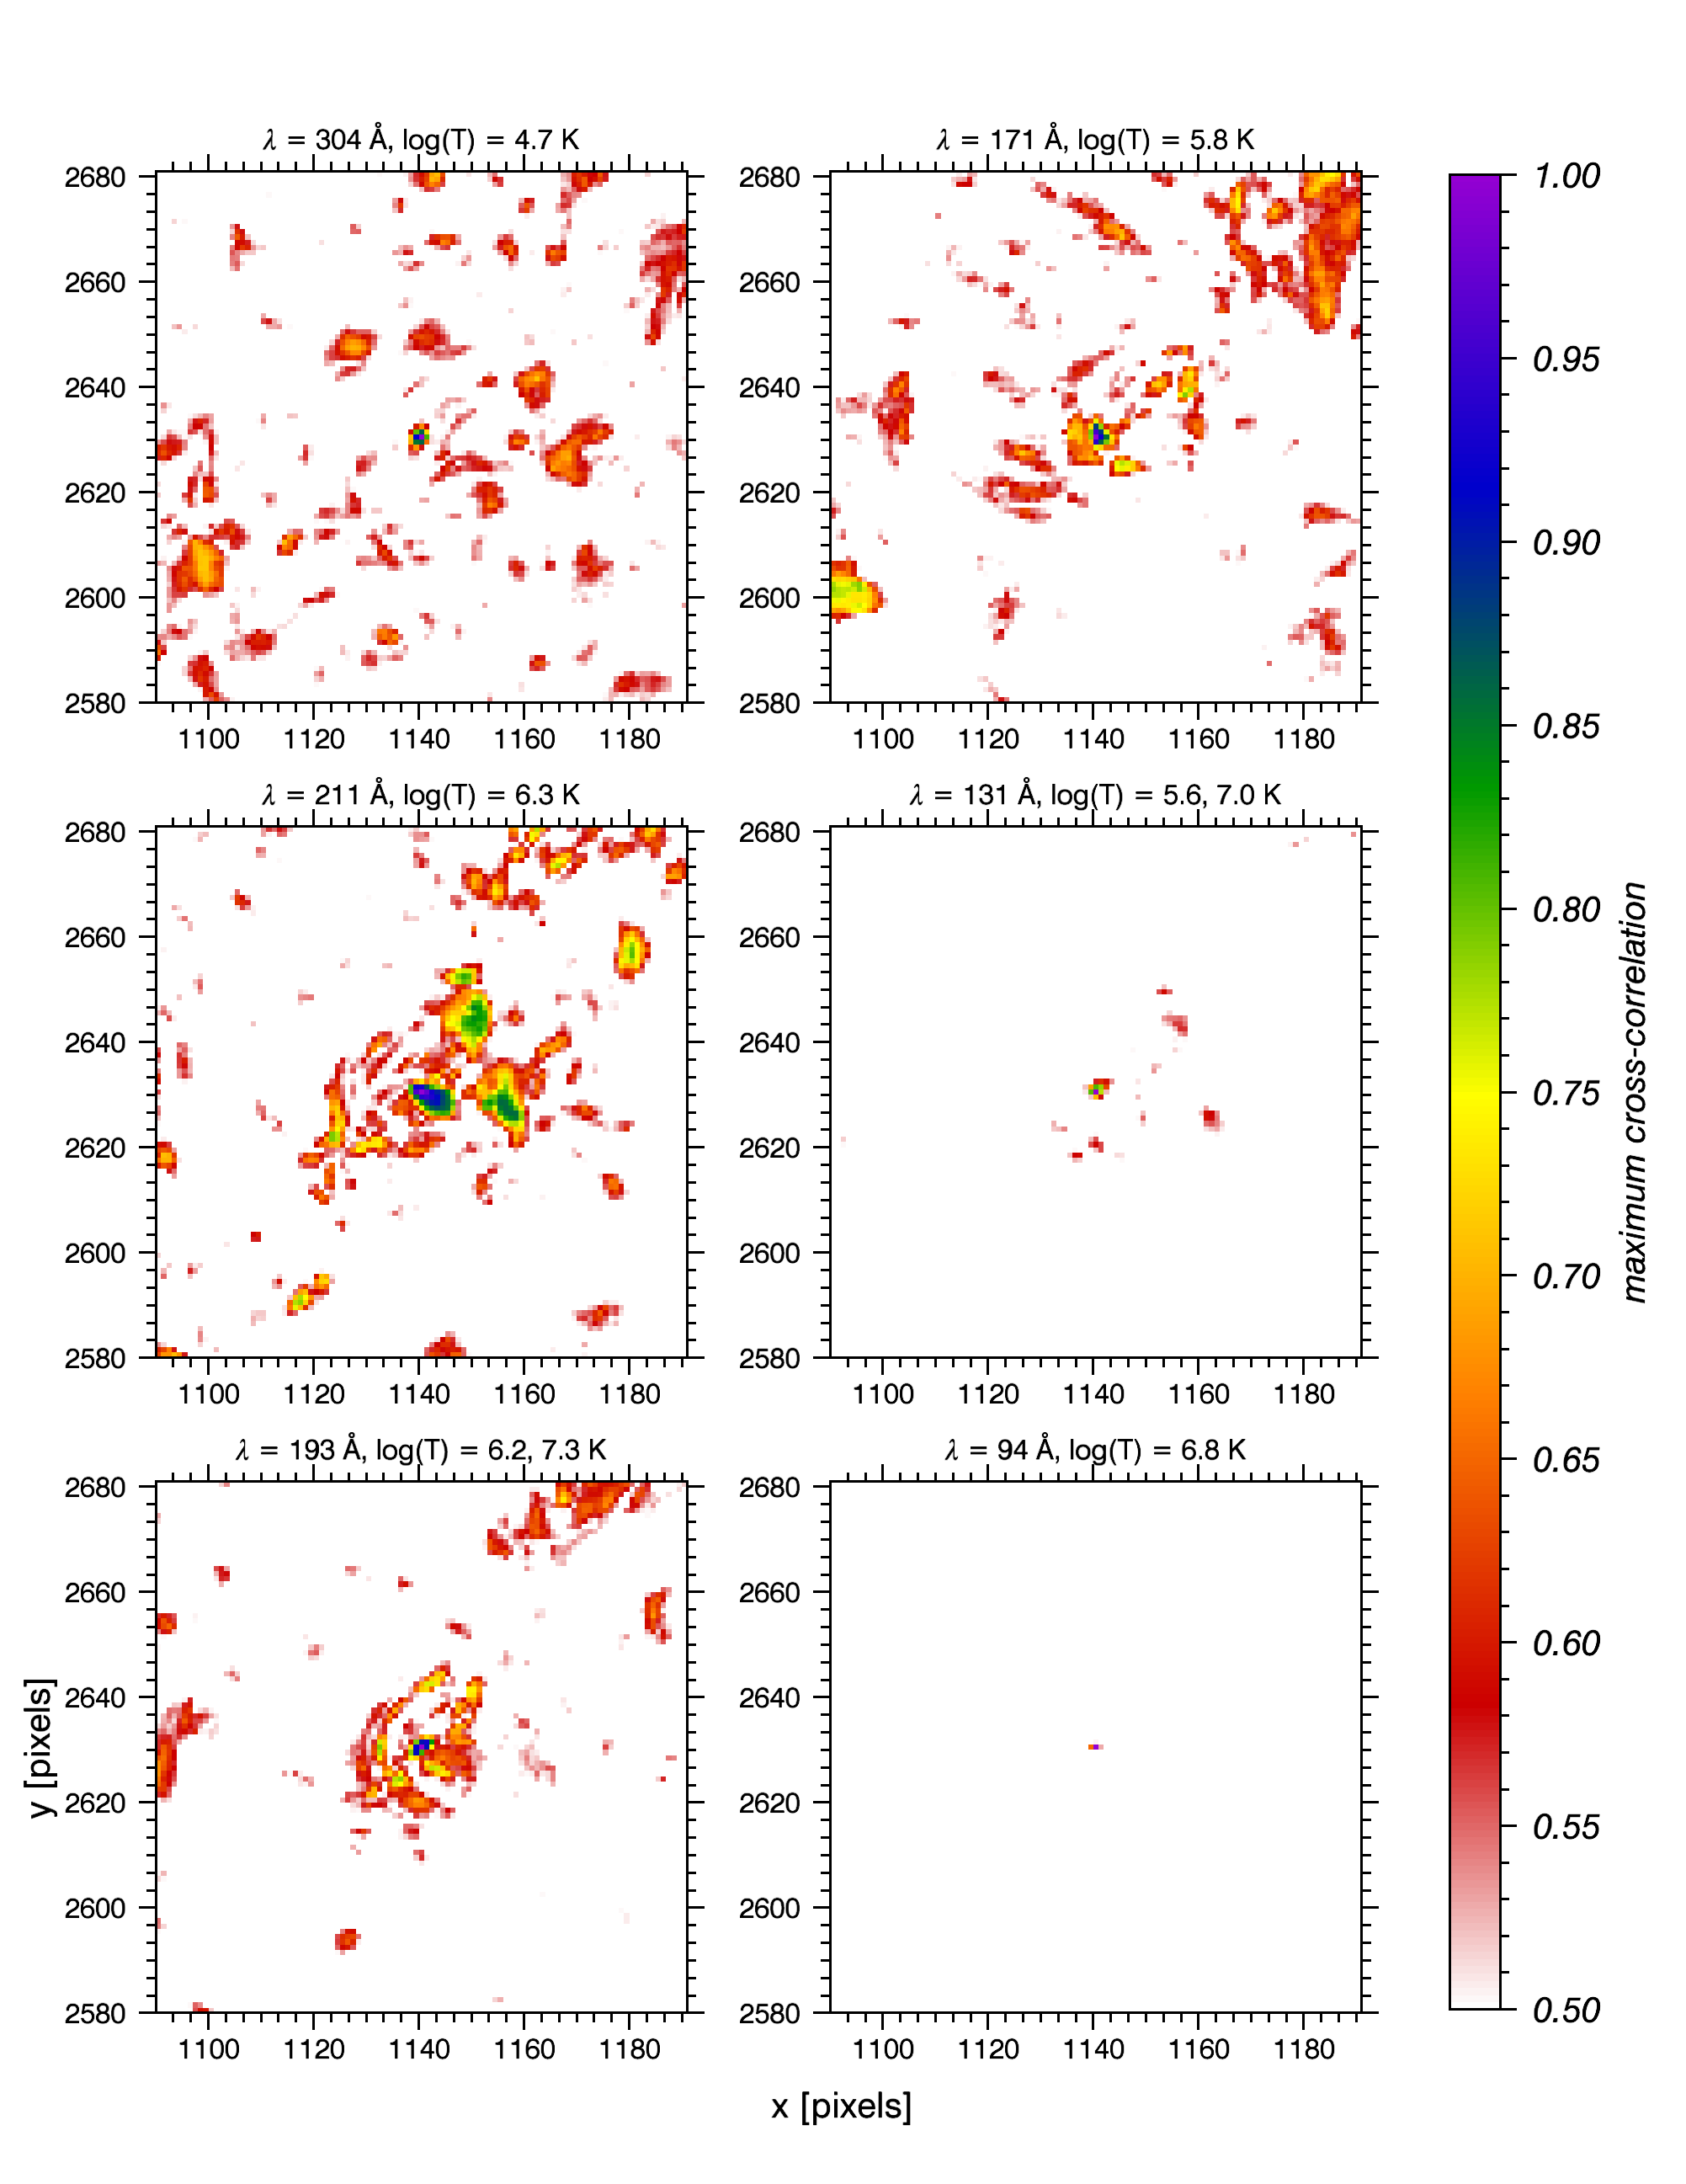
\includegraphics[width=\textwidth]{Figures/cc_images/cc_all_color_cutoff.png}
    \caption{Cross-correlation images scaled to show only values higher than 0.5.}
    \label{cc}
\end{figure*}
\begin{figure*}[htb!]
    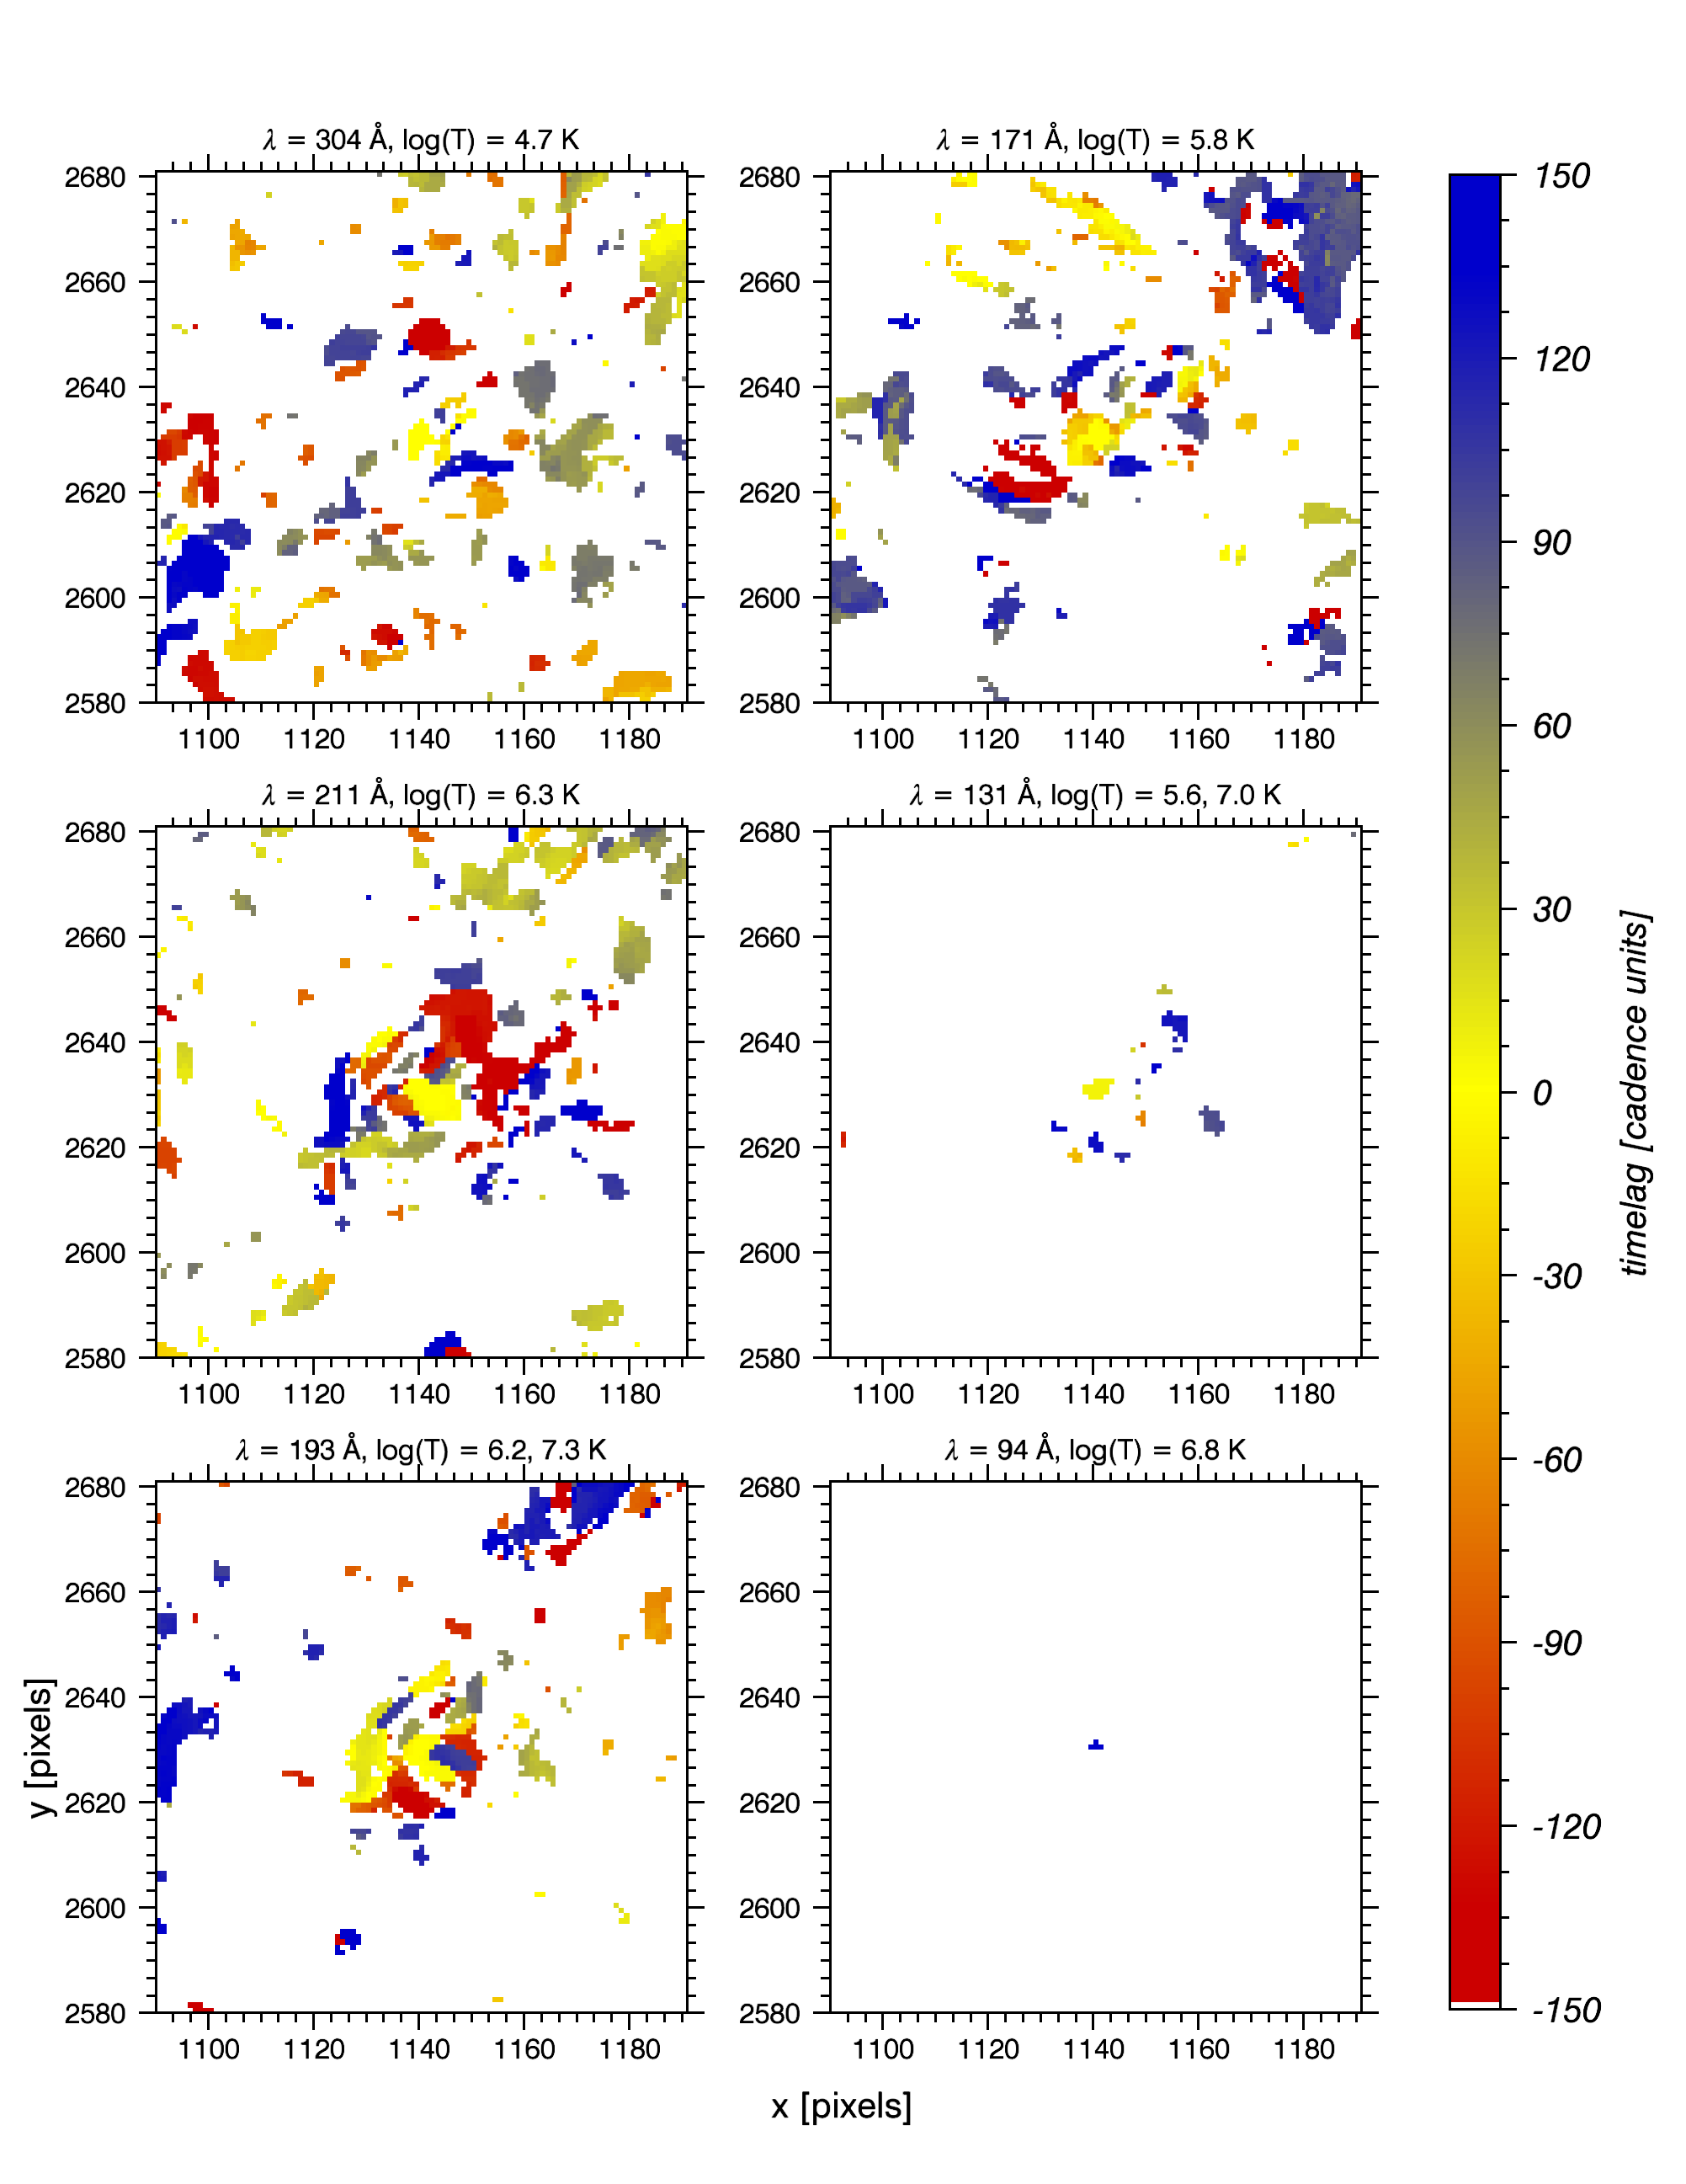
\includegraphics[width=\textwidth]{Figures/tt_images/tt_all_color_cutoff.png}
    \caption{Timelag corresponding to the cross-correlation values higher than 0.5.}
    \label{tt}
\end{figure*}

What does the exact value of cross-correlation tell us? Why would it decrease
from center of BP to the edges? Damping? Directional effects?


\subsection{Variation in BP size with temperature}
Even though the temperature of the corona increases with height from the transition
region to wherever the corona actually ends (need source here), there is not necessarily
a direct correlation between temperature and absolute height above the photosphere
due to the variety of structures
and overall inhomogeneity that exists in the solar atmosphere (\textcolor{red}{source}).
However, the \emph{relative} height between each bandpass for a given structure is
possible to determine, and is relevant to this study.

\subsection{Extra emission in 211\AA{}}
The 211\AA{} data is particularly notable as it shows strong correlation values
at two points to the right of where the BP appears visually in figure \ref{full}.
This could be the result of a jet of light emitted from the main structure, or a
possible indicator of the main structure splitting into several tubes at the
height where the 211 \AA{} emission is strongest.
A movie showing all images from this wavelength
%(\cite{ssw})
revealed a flash
of emission around the 45th image (t = 45*12 seconds),
which matches the timelag at which the high correlation values occurred as shown
in figure \ref{closeup}.

\subsection{Crossing time}
In the corona, the characteristic wave velocity is expected to be close to
the Alfv\'en velocity, which is on the order of 1000 km s$^{-1}$.
\textcolor{darkred}{(With a
cadence of 12 seconds, do we have enough sampling to do this?)}


\begin{figure*}[htb!]
    \includegraphics[width=\textwidth]{Figures/im_211.png}
    \caption{Images from the 211 \AA{} bandpass only, around the times when the
        two jets of light appeared in the upper right region of the main body of the BP. }
    \label{211_images}
\end{figure*}

\begin{figure*}[htb!]
    \includegraphics[width=\textwidth]{Figures/closeup_211.png}
    \caption{Timelag at 211 \AA{} ``zoomed in'' around the two jets of light.}
    \label{closeup}
\end{figure*}

\begin{figure*}[htb!]
    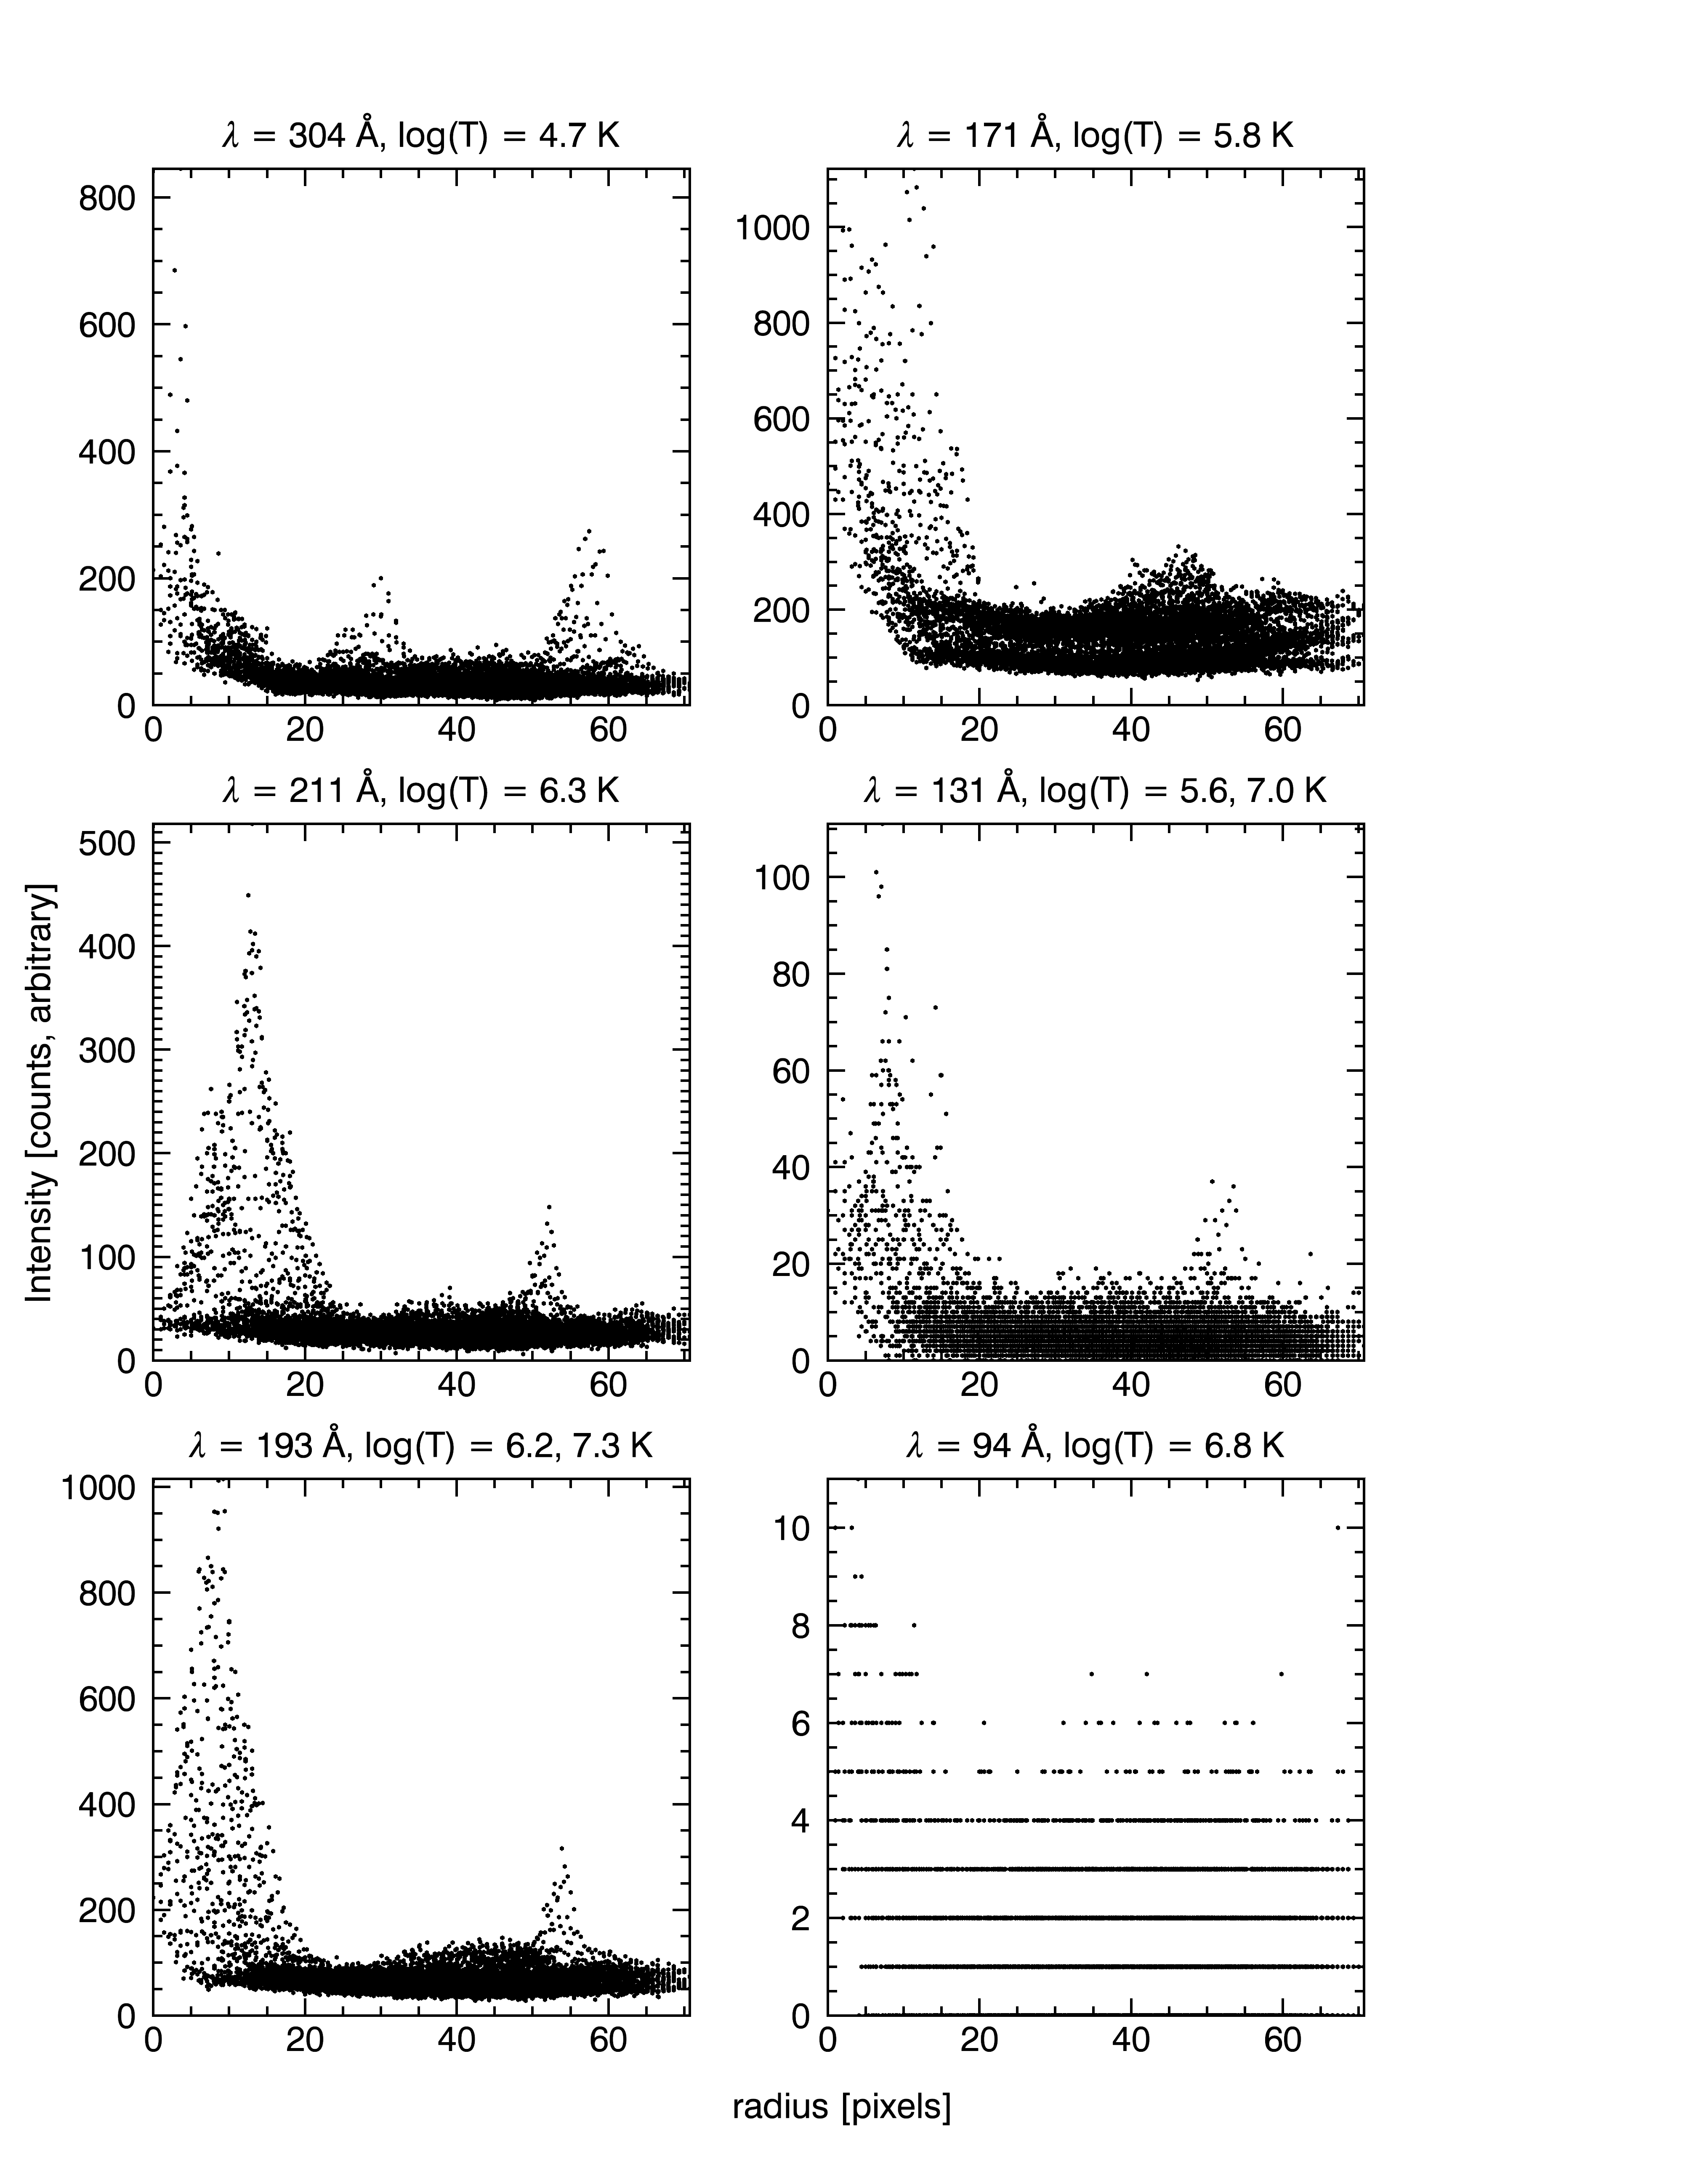
\includegraphics[width=\textwidth]{Figures/intensity_1.png}
    \caption{Intensity of each pixel is plotted as a function of radius for each
        passband. I have no idea what's going on with the 94\AA{} data.}
    \label{intensity_1}
\end{figure*}

\begin{figure*}[htb!]
    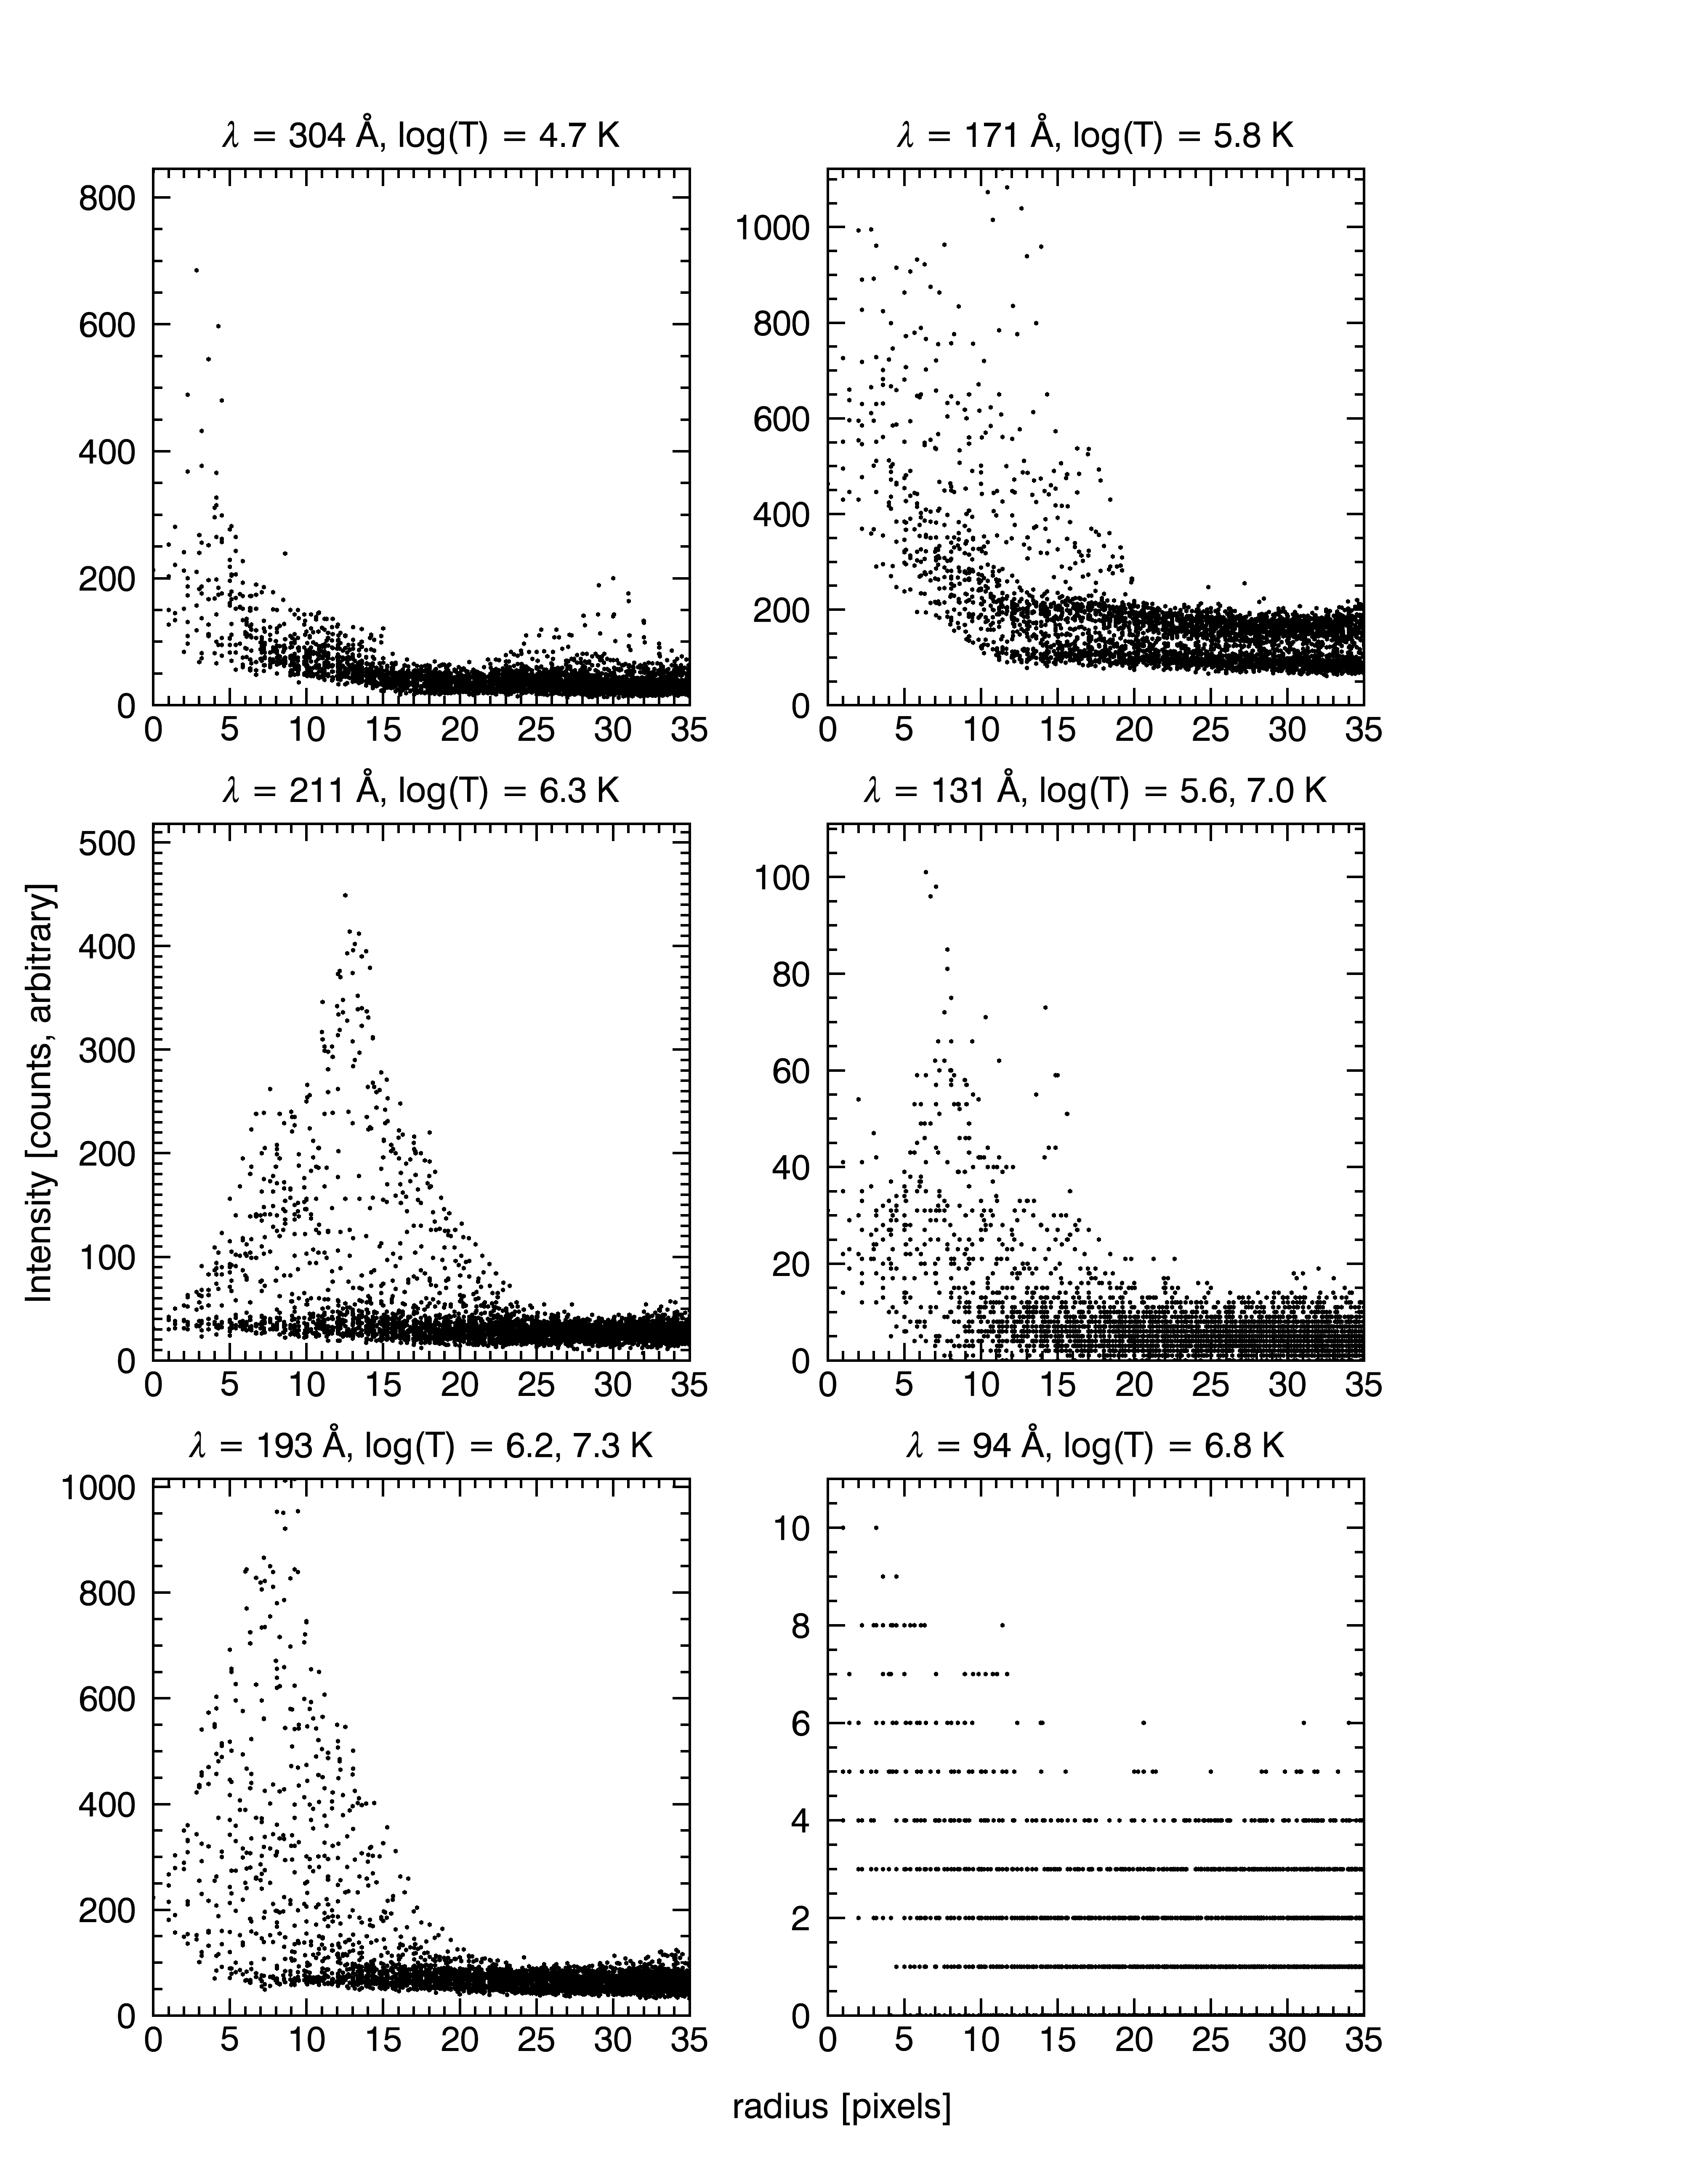
\includegraphics[width=\textwidth]{Figures/intensity_2.png}
    \caption{Same as figure \ref{intensity_1}, but with half the radius range
        cut off to better view the values around the main BP.}
    \label{intensity_2}
\end{figure*}

\begin{figure*}[htb!]
    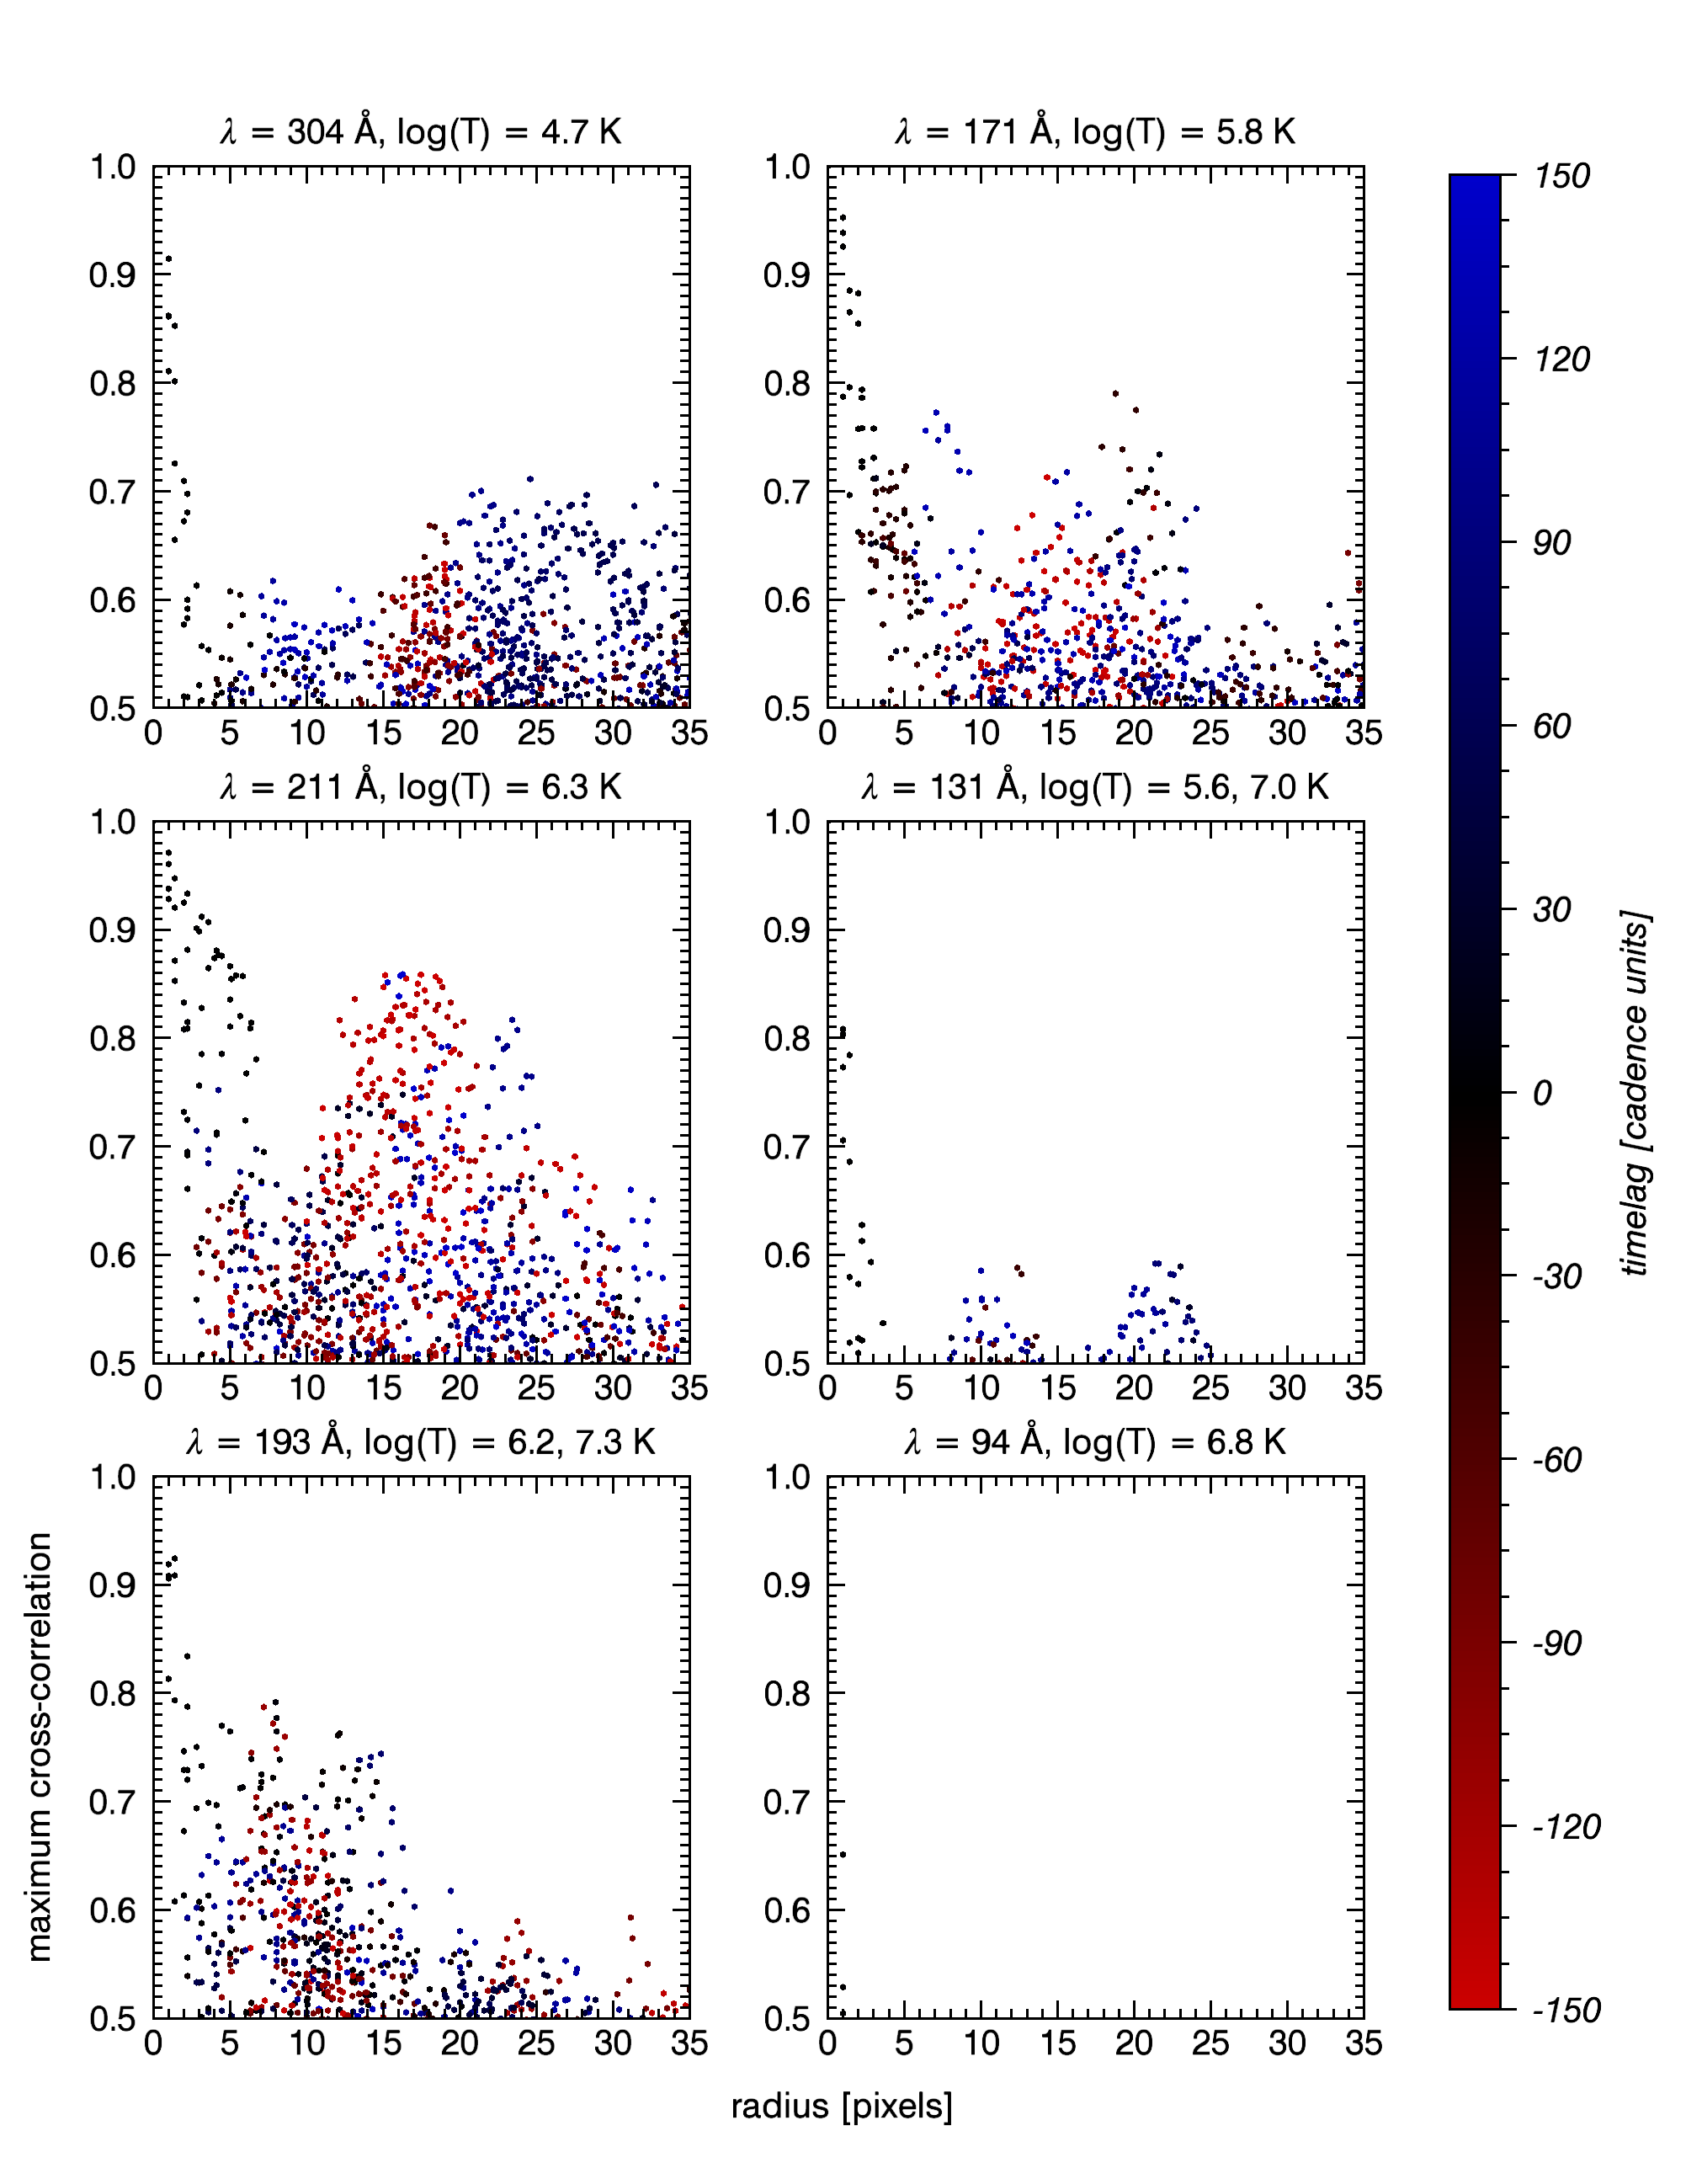
\includegraphics[width=\textwidth]{Figures/cc_tt_plot.png}
    \caption{The highest cross-correlation value of each pixel is plotted as a function
        of its distance from the center pixel. The color indicates the timelag
        corresponding to the maximum cross-correlation for that pixel.}
    \label{tt_all_plot}
\end{figure*}

\begin{figure*}[htb!]
    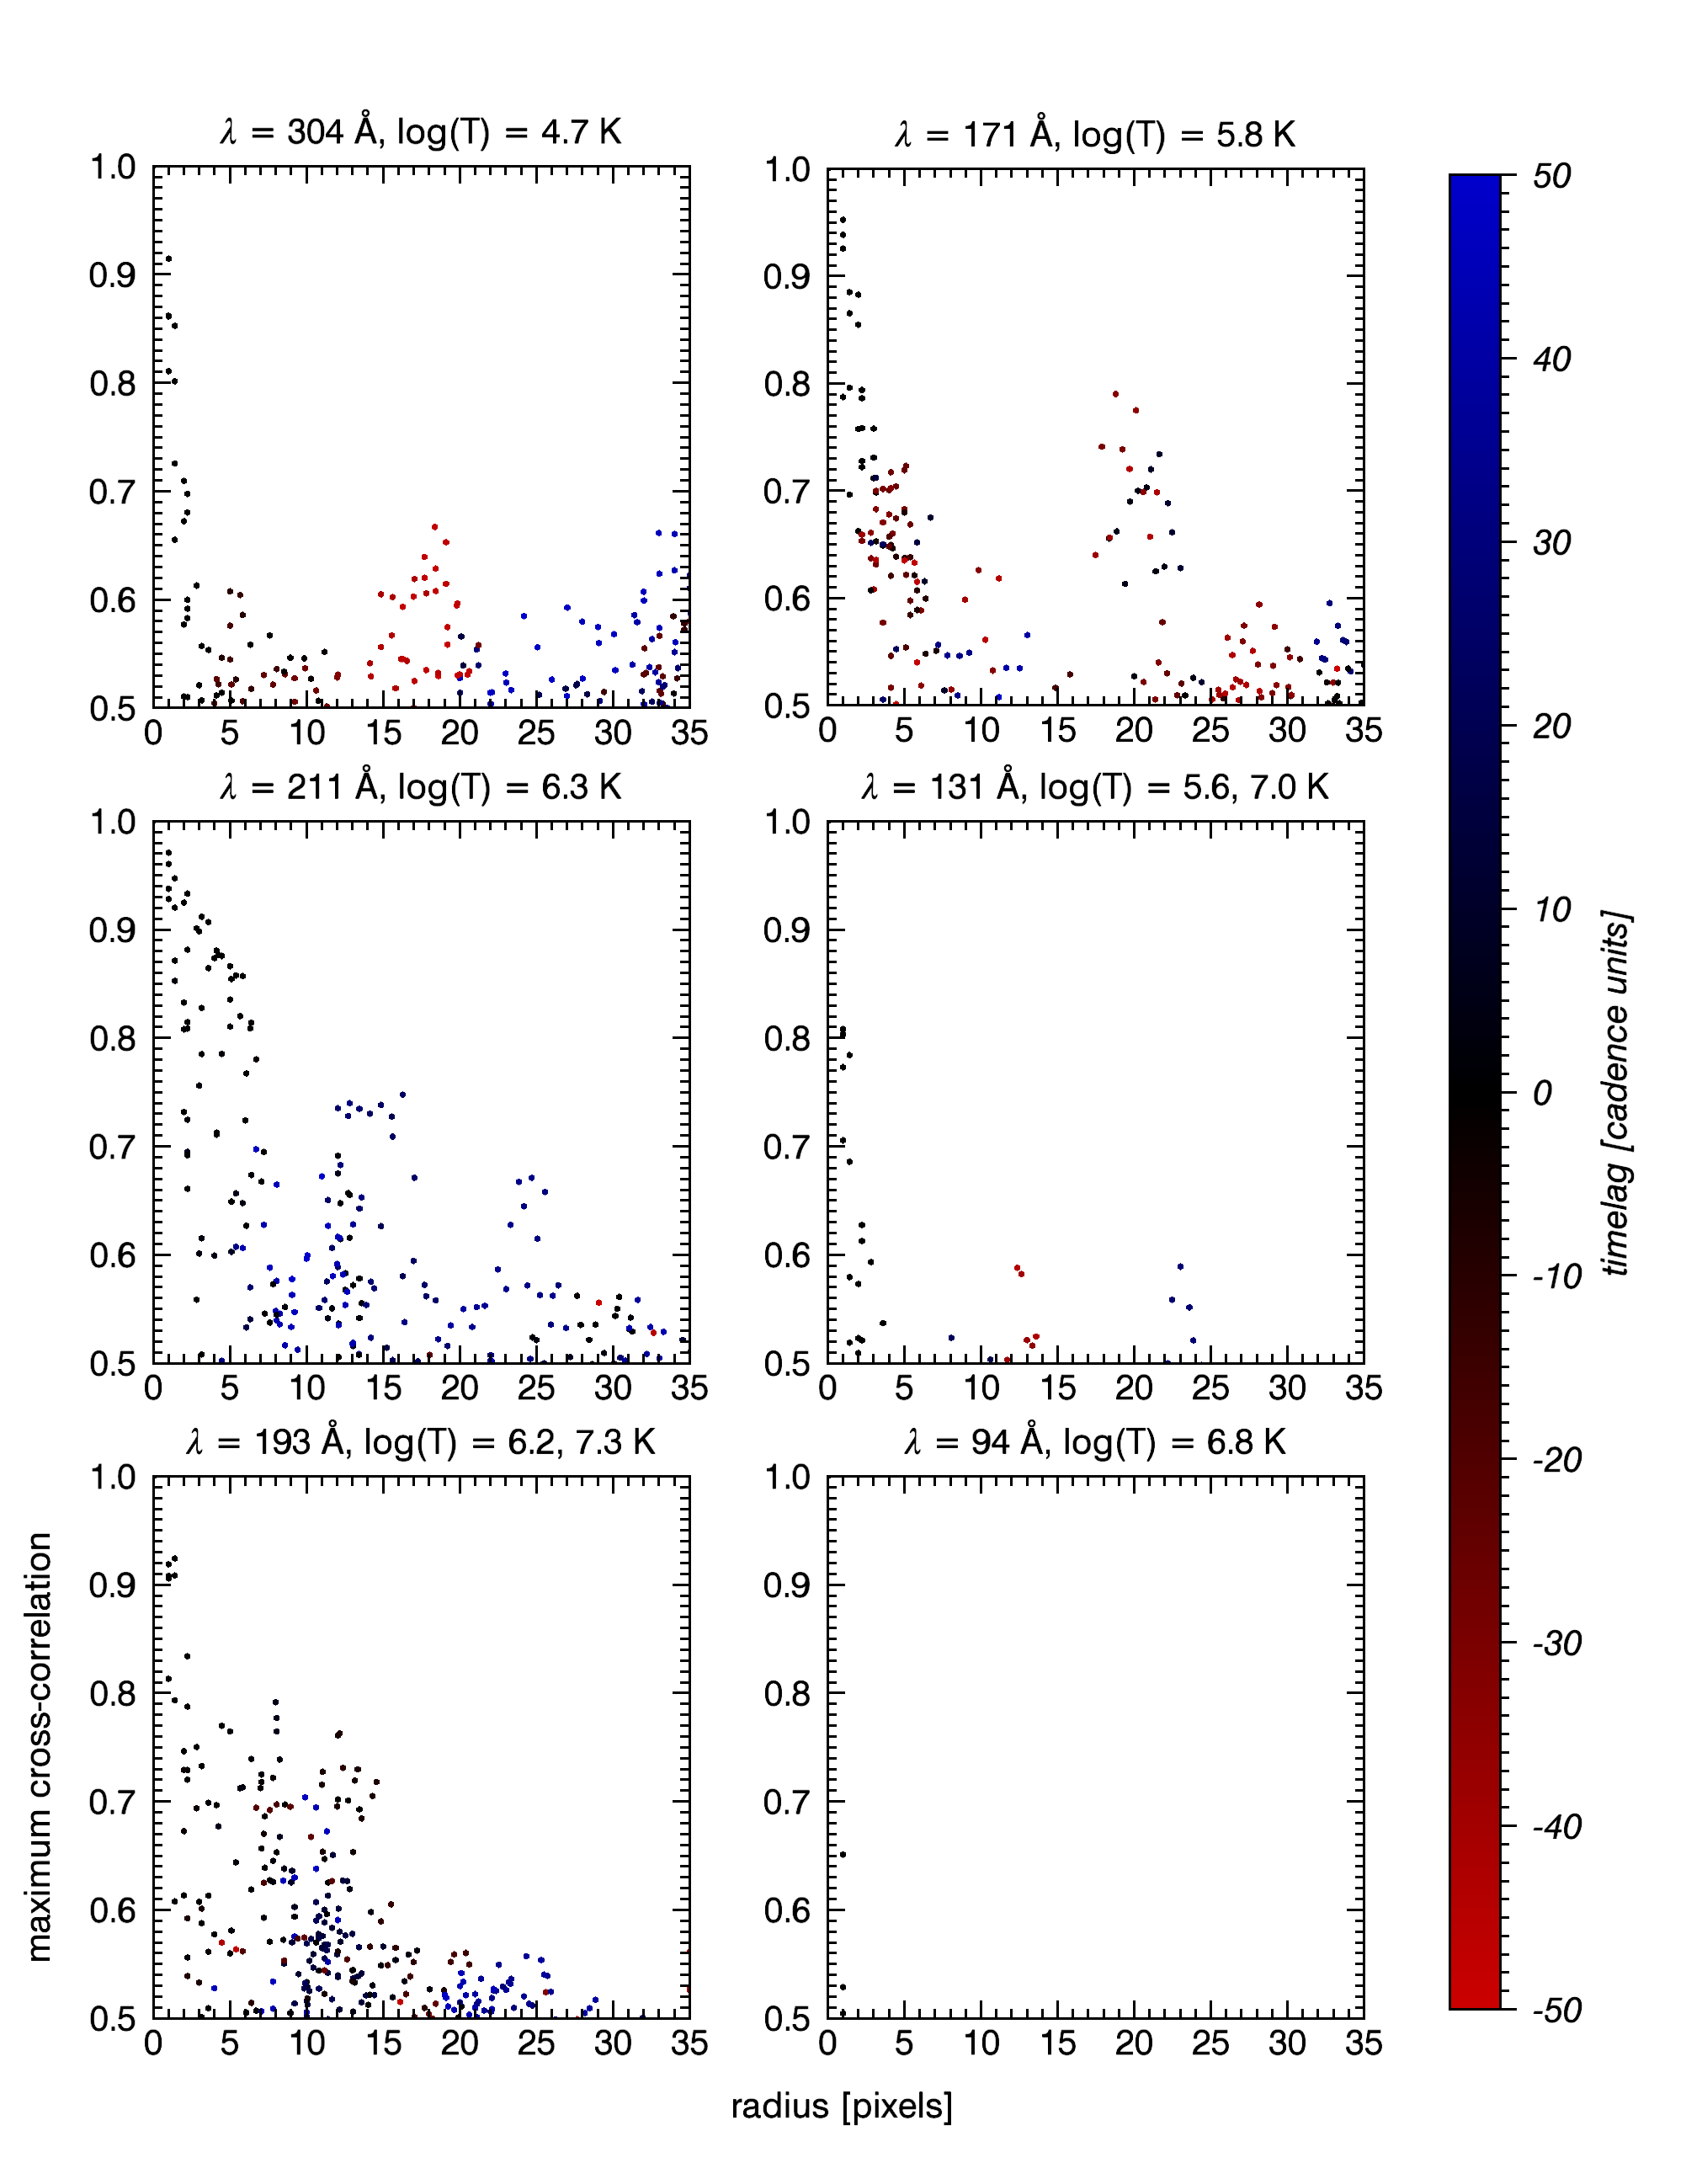
\includegraphics[width=\textwidth]{Figures/cc_tt_plot_scaled.png}
    \caption{Same as figure \ref{tt_all_plot}, but with two thirds of the timelag cut out
        at both ends.}
    \label{tt_plot}
\end{figure*}


\section{Conclusion}\label{conclusion}

\bibliography{reffile}
\end{document}
